\documentclass[a4paper]{book}
\usepackage{makeidx}
\usepackage{natbib}
\usepackage{graphicx}
\usepackage{multicol}
\usepackage{float}
\usepackage{listings}
\usepackage{color}
\usepackage{ifthen}
\usepackage[table]{xcolor}
\usepackage{textcomp}
\usepackage{alltt}
\usepackage{ifpdf}
\ifpdf
\usepackage[pdftex,
            pagebackref=true,
            colorlinks=true,
            linkcolor=blue,
            unicode
           ]{hyperref}
\else
\usepackage[ps2pdf,
            pagebackref=true,
            colorlinks=true,
            linkcolor=blue,
            unicode
           ]{hyperref}
\usepackage{pspicture}
\fi
\usepackage[utf8]{inputenc}
\usepackage{mathptmx}
\usepackage[scaled=.90]{helvet}
\usepackage{courier}
\usepackage{sectsty}
\usepackage[titles]{tocloft}
\usepackage{doxygen}
\lstset{language=C++,inputencoding=utf8,basicstyle=\footnotesize,breaklines=true,breakatwhitespace=true,tabsize=8,numbers=left }
\makeindex
\setcounter{tocdepth}{3}
\renewcommand{\footrulewidth}{0.4pt}
\renewcommand{\familydefault}{\sfdefault}
\hfuzz=15pt
\setlength{\emergencystretch}{15pt}
\hbadness=750
\tolerance=750
\begin{document}
\hypersetup{pageanchor=false,citecolor=blue}
\begin{titlepage}
\vspace*{7cm}
\begin{center}
{\Large \-S\-T\-A\-R\-K \-V\-M\-S }\\
\vspace*{1cm}
{\large \-Generated by Doxygen 1.7.6.1}\\
\vspace*{0.5cm}
{\small Tue Nov 19 2013 16:46:34}\\
\end{center}
\end{titlepage}
\clearemptydoublepage
\pagenumbering{roman}
\tableofcontents
\clearemptydoublepage
\pagenumbering{arabic}
\hypersetup{pageanchor=true,citecolor=blue}
\chapter{\-Namespace \-Index}
\section{\-Namespace \-List}
\-Here is a list of all namespaces with brief descriptions\-:\begin{DoxyCompactList}
\item\contentsline{section}{\hyperlink{namespaceGrammar}{\-Grammar} }{\pageref{d0/da6/namespaceGrammar}}{}
\item\contentsline{section}{\hyperlink{namespaceparser}{parser} }{\pageref{d0/dd5/namespaceparser}}{}
\item\contentsline{section}{\hyperlink{namespacePDA}{\-P\-D\-A} }{\pageref{d7/d11/namespacePDA}}{}
\item\contentsline{section}{\hyperlink{namespaceTM}{\-T\-M} }{\pageref{d6/d65/namespaceTM}}{}
\item\contentsline{section}{\hyperlink{namespaceutilities}{utilities} }{\pageref{d2/d96/namespaceutilities}}{}
\end{DoxyCompactList}

\chapter{\-Class \-Index}
\section{Class Hierarchy}
This inheritance list is sorted roughly, but not completely, alphabetically\-:\begin{DoxyCompactList}
\item \contentsline{section}{C\-F\-G}{\pageref{d7/dd4/classCFG}}{}
\begin{DoxyCompactList}
\item \contentsline{section}{C\-N\-F\-\_\-\-C\-F\-G}{\pageref{da/d5c/classCNF__CFG}}{}
\end{DoxyCompactList}
\item \contentsline{section}{C\-Y\-K\-Table}{\pageref{d6/dcd/classCYKTable}}{}
\item exception\begin{DoxyCompactList}
\item \contentsline{section}{Exception}{\pageref{d4/d67/classException}}{}
\end{DoxyCompactList}
\item \contentsline{section}{Parser}{\pageref{d0/d40/classParser}}{}
\begin{DoxyCompactList}
\item \contentsline{section}{C\-F\-G\-Parser}{\pageref{da/d24/classCFGParser}}{}
\item \contentsline{section}{L\-R\-Parser}{\pageref{d6/de9/classLRParser}}{}
\end{DoxyCompactList}
\item \contentsline{section}{Parse\-Table}{\pageref{d9/da1/classParseTable}}{}
\item \contentsline{section}{P\-D\-A\-:\-:P\-D\-A}{\pageref{d1/dc5/classPDA_1_1PDA}}{}
\item \contentsline{section}{P\-D\-A\-:\-:State}{\pageref{d7/d1f/classPDA_1_1State}}{}
\end{DoxyCompactList}

\chapter{\-Class \-Index}
\section{\-Class \-List}
\-Here are the classes, structs, unions and interfaces with brief descriptions\-:\begin{DoxyCompactList}
\item\contentsline{section}{\hyperlink{classCFG}{\-C\-F\-G} }{\pageref{d7/dd4/classCFG}}{}
\item\contentsline{section}{\hyperlink{classCFGParser}{\-C\-F\-G\-Parser} }{\pageref{da/d24/classCFGParser}}{}
\item\contentsline{section}{\hyperlink{classCNF__CFG}{\-C\-N\-F\-\_\-\-C\-F\-G} }{\pageref{da/d5c/classCNF__CFG}}{}
\item\contentsline{section}{\hyperlink{classCYKTable}{\-C\-Y\-K\-Table} }{\pageref{d6/dcd/classCYKTable}}{}
\item\contentsline{section}{\hyperlink{classException}{\-Exception} }{\pageref{d4/d67/classException}}{}
\item\contentsline{section}{\hyperlink{classLRParser}{\-L\-R\-Parser} }{\pageref{d6/de9/classLRParser}}{}
\item\contentsline{section}{\hyperlink{classParser}{\-Parser} }{\pageref{d0/d40/classParser}}{}
\item\contentsline{section}{\hyperlink{classParseTable}{\-Parse\-Table} }{\pageref{d9/da1/classParseTable}}{}
\item\contentsline{section}{\hyperlink{classPDA_1_1PDA}{\-P\-D\-A\-::\-P\-D\-A} }{\pageref{d1/dc5/classPDA_1_1PDA}}{}
\item\contentsline{section}{\hyperlink{classPDA_1_1State}{\-P\-D\-A\-::\-State} }{\pageref{d7/d1f/classPDA_1_1State}}{}
\end{DoxyCompactList}

\chapter{\-File \-Index}
\section{\-File \-List}
\-Here is a list of all files with brief descriptions\-:\begin{DoxyCompactList}
\item\contentsline{section}{src/\hyperlink{CFG_8h}{\-C\-F\-G.\-h} }{\pageref{d9/d25/CFG_8h}}{}
\item\contentsline{section}{src/\hyperlink{CYKTable_8h}{\-C\-Y\-K\-Table.\-h} }{\pageref{db/d5c/CYKTable_8h}}{}
\item\contentsline{section}{src/\hyperlink{DesignByContract_8h}{\-Design\-By\-Contract.\-h} }{\pageref{d0/d30/DesignByContract_8h}}{}
\item\contentsline{section}{src/\hyperlink{Exception_8h}{\-Exception.\-h} }{\pageref{d8/d8a/Exception_8h}}{}
\item\contentsline{section}{src/\hyperlink{Information_8h}{\-Information.\-h} }{\pageref{d6/d92/Information_8h}}{}
\item\contentsline{section}{src/\hyperlink{LRParser_8h}{\-L\-R\-Parser.\-h} }{\pageref{de/db3/LRParser_8h}}{}
\item\contentsline{section}{src/\hyperlink{Parser_8h}{\-Parser.\-h} }{\pageref{d6/d0c/Parser_8h}}{}
\item\contentsline{section}{src/\hyperlink{ParseTable_8h}{\-Parse\-Table.\-h} }{\pageref{d4/d97/ParseTable_8h}}{}
\item\contentsline{section}{src/\hyperlink{PDA_8h}{\-P\-D\-A.\-h} }{\pageref{d5/d4a/PDA_8h}}{}
\item\contentsline{section}{src/\hyperlink{State_8h}{\-State.\-h} }{\pageref{dd/d99/State_8h}}{}
\item\contentsline{section}{src/\hyperlink{TMParser_8h}{\-T\-M\-Parser.\-h} }{\pageref{d9/d25/TMParser_8h}}{}
\item\contentsline{section}{src/\hyperlink{TuringMachine_8h}{\-Turing\-Machine.\-h} }{\pageref{d1/d44/TuringMachine_8h}}{}
\item\contentsline{section}{src/\hyperlink{utilities_8h}{utilities.\-h} }{\pageref{de/df0/utilities_8h}}{}
\end{DoxyCompactList}

\chapter{\-Namespace \-Documentation}
\hypertarget{namespacePDA}{\section{\-P\-D\-A \-Namespace \-Reference}
\label{d7/d11/namespacePDA}\index{\-P\-D\-A@{\-P\-D\-A}}
}
\subsection*{\-Classes}
\begin{DoxyCompactItemize}
\item 
class \hyperlink{classPDA_1_1PDA}{\-P\-D\-A}
\item 
class \hyperlink{classPDA_1_1State}{\-State}
\end{DoxyCompactItemize}
\subsection*{\-Enumerations}
\begin{DoxyCompactItemize}
\item 
enum \hyperlink{namespacePDA_a2f2b17cdf30facf6f0fe593ab209acf8}{\-P\-D\-A\-Type} \{ \hyperlink{namespacePDA_a2f2b17cdf30facf6f0fe593ab209acf8abec96ee068d9af07a9bf41137e3b3635}{accept\-By\-Empty\-Stack}, 
\hyperlink{namespacePDA_a2f2b17cdf30facf6f0fe593ab209acf8a68e7e330c1fb2405ce07c4f2600139e1}{accept\-By\-Final\-State}
 \}
\end{DoxyCompactItemize}


\subsection{\-Enumeration \-Type \-Documentation}
\hypertarget{namespacePDA_a2f2b17cdf30facf6f0fe593ab209acf8}{\index{\-P\-D\-A@{\-P\-D\-A}!\-P\-D\-A\-Type@{\-P\-D\-A\-Type}}
\index{\-P\-D\-A\-Type@{\-P\-D\-A\-Type}!PDA@{\-P\-D\-A}}
\subsubsection[{\-P\-D\-A\-Type}]{\setlength{\rightskip}{0pt plus 5cm}enum {\bf \-P\-D\-A\-::\-P\-D\-A\-Type}}}\label{d7/d11/namespacePDA_a2f2b17cdf30facf6f0fe593ab209acf8}
\begin{Desc}
\item[\-Enumerator\-: ]\par
\begin{description}
\index{accept\-By\-Empty\-Stack@{accept\-By\-Empty\-Stack}!\-P\-D\-A@{\-P\-D\-A}}\index{\-P\-D\-A@{\-P\-D\-A}!accept\-By\-Empty\-Stack@{accept\-By\-Empty\-Stack}}\item[{\em 
\hypertarget{namespacePDA_a2f2b17cdf30facf6f0fe593ab209acf8abec96ee068d9af07a9bf41137e3b3635}{accept\-By\-Empty\-Stack}\label{d7/d11/namespacePDA_a2f2b17cdf30facf6f0fe593ab209acf8abec96ee068d9af07a9bf41137e3b3635}
}]\index{accept\-By\-Final\-State@{accept\-By\-Final\-State}!\-P\-D\-A@{\-P\-D\-A}}\index{\-P\-D\-A@{\-P\-D\-A}!accept\-By\-Final\-State@{accept\-By\-Final\-State}}\item[{\em 
\hypertarget{namespacePDA_a2f2b17cdf30facf6f0fe593ab209acf8a68e7e330c1fb2405ce07c4f2600139e1}{accept\-By\-Final\-State}\label{d7/d11/namespacePDA_a2f2b17cdf30facf6f0fe593ab209acf8a68e7e330c1fb2405ce07c4f2600139e1}
}]\end{description}
\end{Desc}


\hypertarget{namespaceutilities}{\section{utilities Namespace Reference}
\label{namespaceutilities}\index{utilities@{utilities}}
}
\subsection*{Functions}
\begin{DoxyCompactItemize}
\item 
bool \hyperlink{namespaceutilities_a620604f61984de35f2aadb90f37c7648}{is\-Number} (std\-::string)
\item 
std\-::string \hyperlink{namespaceutilities_a937f243bd57e4a94510304c6a9920064}{char\-To\-String} (char)
\end{DoxyCompactItemize}


\subsection{Function Documentation}
\hypertarget{namespaceutilities_a937f243bd57e4a94510304c6a9920064}{\index{utilities@{utilities}!char\-To\-String@{char\-To\-String}}
\index{char\-To\-String@{char\-To\-String}!utilities@{utilities}}
\subsubsection[{char\-To\-String}]{\setlength{\rightskip}{0pt plus 5cm}std\-::string utilities\-::char\-To\-String (
\begin{DoxyParamCaption}
\item[{char}]{}
\end{DoxyParamCaption}
)}}\label{namespaceutilities_a937f243bd57e4a94510304c6a9920064}
\hypertarget{namespaceutilities_a620604f61984de35f2aadb90f37c7648}{\index{utilities@{utilities}!is\-Number@{is\-Number}}
\index{is\-Number@{is\-Number}!utilities@{utilities}}
\subsubsection[{is\-Number}]{\setlength{\rightskip}{0pt plus 5cm}bool utilities\-::is\-Number (
\begin{DoxyParamCaption}
\item[{std\-::string}]{}
\end{DoxyParamCaption}
)}}\label{namespaceutilities_a620604f61984de35f2aadb90f37c7648}

\chapter{\-Class \-Documentation}
\hypertarget{classCFG}{\section{\-C\-F\-G \-Class \-Reference}
\label{d7/dd4/classCFG}\index{\-C\-F\-G@{\-C\-F\-G}}
}


{\ttfamily \#include $<$\-C\-F\-G.\-h$>$}

\-Inheritance diagram for \-C\-F\-G\-:\begin{figure}[H]
\begin{center}
\leavevmode
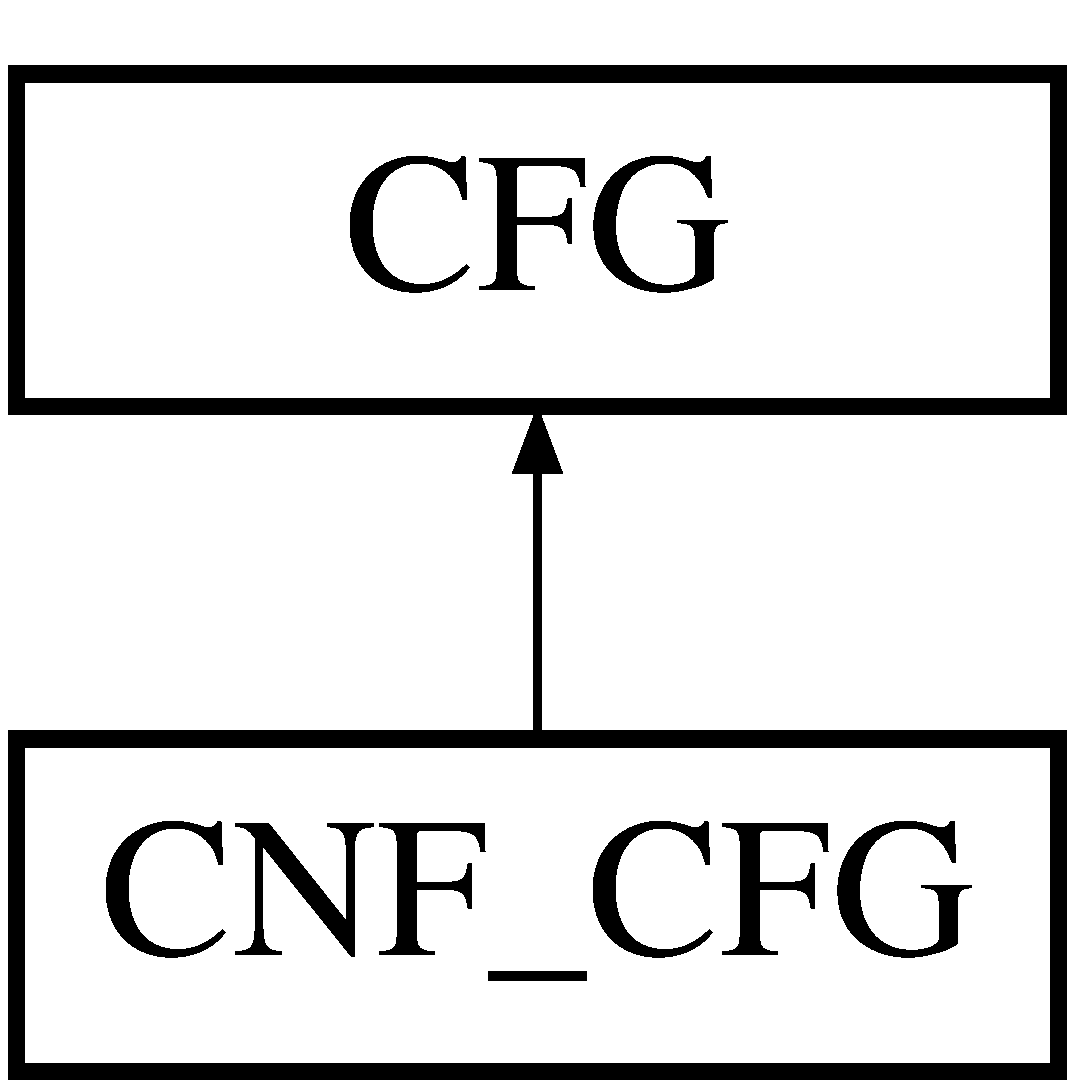
\includegraphics[height=2.000000cm]{d7/dd4/classCFG}
\end{center}
\end{figure}
\subsection*{\-Public \-Member \-Functions}
\begin{DoxyCompactItemize}
\item 
\hyperlink{classCFG_a6a6d74b60d6abc9b91031aaac23067ff}{\-C\-F\-G} ()
\begin{DoxyCompactList}\small\item\em \-Default constructor. \end{DoxyCompactList}\item 
\hyperlink{classCFG_ae6f918a908ebef14199ce1e6ce909196}{\-C\-F\-G} (std\-::vector$<$ std\-::string $>$ \&v, std\-::vector$<$ std\-::string $>$ \&t, std\-::map$<$ std\-::string, std\-::vector$<$ std\-::string $>$ $>$ \&r, std\-::string s)
\begin{DoxyCompactList}\small\item\em specified constructor \end{DoxyCompactList}\item 
\hyperlink{classCFG_a5a7524ec649377e2d8c2d8218db40b44}{\-C\-F\-G} (std\-::string file)
\begin{DoxyCompactList}\small\item\em \-Constructor from a given file. \end{DoxyCompactList}\item 
\hyperlink{classCFG_acdf5e087e7726343079e006f6dd0d43e}{\-C\-F\-G} (\hyperlink{classCFG}{\-C\-F\-G} \&copy)
\begin{DoxyCompactList}\small\item\em \-Copy constructor. \end{DoxyCompactList}\item 
void \hyperlink{classCFG_a4f0a00a699ba4a6247333a47b0bf9ff2}{to\-C\-N\-F} ()
\item 
std\-::vector$<$ std\-::string $>$ \hyperlink{classCFG_abe3e4a8324808575d5d0c033671b71ab}{get\-Variables} () const 
\item 
std\-::vector$<$ std\-::string $>$ \hyperlink{classCFG_a766b9baac4bd283b8b761139e75aae55}{get\-Terminals} () const 
\item 
std\-::map$<$ std\-::string, \*
std\-::vector$<$ std\-::string $>$ $>$ \hyperlink{classCFG_aa861ae80a1391594cf2bf50cfac38ea9}{get\-Rules} () const 
\item 
std\-::string \hyperlink{classCFG_ae7e150fabee50d533159038262bc71d3}{get\-Start} () const 
\item 
virtual \hyperlink{classCFG_aaf69bdb0d01010bf6272a097ccc0c60c}{$\sim$\-C\-F\-G} ()
\end{DoxyCompactItemize}
\subsection*{\-Protected \-Member \-Functions}
\begin{DoxyCompactItemize}
\item 
void \hyperlink{classCFG_a20c962c9056a1770d71f9610df8db905}{check\-Attributes} ()
\begin{DoxyCompactList}\small\item\em the start symbol of the \hyperlink{classCFG}{\-C\-F\-G} \end{DoxyCompactList}\end{DoxyCompactItemize}
\subsection*{\-Protected \-Attributes}
\begin{DoxyCompactItemize}
\item 
std\-::vector$<$ std\-::string $>$ \hyperlink{classCFG_a7369373d17b20520d7b72d43f471cda9}{variables\-\_\-}
\item 
std\-::vector$<$ std\-::string $>$ \hyperlink{classCFG_ac105b578d6237fc6ff28e54c98bbb1b8}{terminals\-\_\-}
\begin{DoxyCompactList}\small\item\em vector with the variables of the \hyperlink{classCFG}{\-C\-F\-G} \end{DoxyCompactList}\item 
std\-::map$<$ std\-::string, \*
std\-::vector$<$ std\-::string $>$ $>$ \hyperlink{classCFG_a6f148c60599eec412d168d2353b7b814}{rules\-\_\-}
\begin{DoxyCompactList}\small\item\em vector with the terminals of the \hyperlink{classCFG}{\-C\-F\-G} \end{DoxyCompactList}\item 
std\-::string \hyperlink{classCFG_a21527e2ffbb0b5bf8995ebae725858eb}{start\-Symbol\-\_\-}
\begin{DoxyCompactList}\small\item\em a map with all the rules. rules are of the form $<$\-Variable$>$, vector$<$\-Variables, terminals$>$ \end{DoxyCompactList}\end{DoxyCompactItemize}
\subsection*{\-Friends}
\begin{DoxyCompactItemize}
\item 
std\-::ostream \& \hyperlink{classCFG_a125cf827399aa731591064e741ab8fb7}{operator$<$$<$} (std\-::ostream \&out, \hyperlink{classCFG}{\-C\-F\-G} \&c)
\begin{DoxyCompactList}\small\item\em output operator \end{DoxyCompactList}\end{DoxyCompactItemize}


\subsection{\-Constructor \& \-Destructor \-Documentation}
\hypertarget{classCFG_a6a6d74b60d6abc9b91031aaac23067ff}{\index{\-C\-F\-G@{\-C\-F\-G}!\-C\-F\-G@{\-C\-F\-G}}
\index{\-C\-F\-G@{\-C\-F\-G}!CFG@{\-C\-F\-G}}
\subsubsection[{\-C\-F\-G}]{\setlength{\rightskip}{0pt plus 5cm}{\bf \-C\-F\-G\-::\-C\-F\-G} (
\begin{DoxyParamCaption}
{}
\end{DoxyParamCaption}
)}}\label{d7/dd4/classCFG_a6a6d74b60d6abc9b91031aaac23067ff}


\-Default constructor. 

\hypertarget{classCFG_ae6f918a908ebef14199ce1e6ce909196}{\index{\-C\-F\-G@{\-C\-F\-G}!\-C\-F\-G@{\-C\-F\-G}}
\index{\-C\-F\-G@{\-C\-F\-G}!CFG@{\-C\-F\-G}}
\subsubsection[{\-C\-F\-G}]{\setlength{\rightskip}{0pt plus 5cm}{\bf \-C\-F\-G\-::\-C\-F\-G} (
\begin{DoxyParamCaption}
\item[{std\-::vector$<$ std\-::string $>$ \&}]{v, }
\item[{std\-::vector$<$ std\-::string $>$ \&}]{t, }
\item[{std\-::map$<$ std\-::string, std\-::vector$<$ std\-::string $>$ $>$ \&}]{r, }
\item[{std\-::string}]{s}
\end{DoxyParamCaption}
)}}\label{d7/dd4/classCFG_ae6f918a908ebef14199ce1e6ce909196}


specified constructor 


\begin{DoxyParams}{\-Parameters}
{\em v} & vector with variables \\
\hline
{\em t} & vector with terminals \\
\hline
{\em r} & map with rules of the form $<$\-Variable$>$, vector$<$terminals,\-Variables$>$ \\
\hline
{\em s} & the start symbol for the \hyperlink{classCFG}{\-C\-F\-G} \\
\hline
\end{DoxyParams}
\hypertarget{classCFG_a5a7524ec649377e2d8c2d8218db40b44}{\index{\-C\-F\-G@{\-C\-F\-G}!\-C\-F\-G@{\-C\-F\-G}}
\index{\-C\-F\-G@{\-C\-F\-G}!CFG@{\-C\-F\-G}}
\subsubsection[{\-C\-F\-G}]{\setlength{\rightskip}{0pt plus 5cm}{\bf \-C\-F\-G\-::\-C\-F\-G} (
\begin{DoxyParamCaption}
\item[{std\-::string}]{file}
\end{DoxyParamCaption}
)}}\label{d7/dd4/classCFG_a5a7524ec649377e2d8c2d8218db40b44}


\-Constructor from a given file. 


\begin{DoxyParams}{\-Parameters}
{\em file} & the path to a file where the \hyperlink{classCFG}{\-C\-F\-G} is described \\
\hline
\end{DoxyParams}
\hypertarget{classCFG_acdf5e087e7726343079e006f6dd0d43e}{\index{\-C\-F\-G@{\-C\-F\-G}!\-C\-F\-G@{\-C\-F\-G}}
\index{\-C\-F\-G@{\-C\-F\-G}!CFG@{\-C\-F\-G}}
\subsubsection[{\-C\-F\-G}]{\setlength{\rightskip}{0pt plus 5cm}{\bf \-C\-F\-G\-::\-C\-F\-G} (
\begin{DoxyParamCaption}
\item[{{\bf \-C\-F\-G} \&}]{copy}
\end{DoxyParamCaption}
)}}\label{d7/dd4/classCFG_acdf5e087e7726343079e006f6dd0d43e}


\-Copy constructor. 


\begin{DoxyParams}{\-Parameters}
{\em copy} & a \hyperlink{classCFG}{\-C\-F\-G} object which is going to be copied \\
\hline
\end{DoxyParams}
\hypertarget{classCFG_aaf69bdb0d01010bf6272a097ccc0c60c}{\index{\-C\-F\-G@{\-C\-F\-G}!$\sim$\-C\-F\-G@{$\sim$\-C\-F\-G}}
\index{$\sim$\-C\-F\-G@{$\sim$\-C\-F\-G}!CFG@{\-C\-F\-G}}
\subsubsection[{$\sim$\-C\-F\-G}]{\setlength{\rightskip}{0pt plus 5cm}virtual {\bf \-C\-F\-G\-::$\sim$\-C\-F\-G} (
\begin{DoxyParamCaption}
{}
\end{DoxyParamCaption}
)\hspace{0.3cm}{\ttfamily  \mbox{[}virtual\mbox{]}}}}\label{d7/dd4/classCFG_aaf69bdb0d01010bf6272a097ccc0c60c}


\subsection{\-Member \-Function \-Documentation}
\hypertarget{classCFG_a20c962c9056a1770d71f9610df8db905}{\index{\-C\-F\-G@{\-C\-F\-G}!check\-Attributes@{check\-Attributes}}
\index{check\-Attributes@{check\-Attributes}!CFG@{\-C\-F\-G}}
\subsubsection[{check\-Attributes}]{\setlength{\rightskip}{0pt plus 5cm}void {\bf \-C\-F\-G\-::check\-Attributes} (
\begin{DoxyParamCaption}
{}
\end{DoxyParamCaption}
)\hspace{0.3cm}{\ttfamily  \mbox{[}protected\mbox{]}}}}\label{d7/dd4/classCFG_a20c962c9056a1770d71f9610df8db905}


the start symbol of the \hyperlink{classCFG}{\-C\-F\-G} 

checks whether all attributes are ok \hypertarget{classCFG_aa861ae80a1391594cf2bf50cfac38ea9}{\index{\-C\-F\-G@{\-C\-F\-G}!get\-Rules@{get\-Rules}}
\index{get\-Rules@{get\-Rules}!CFG@{\-C\-F\-G}}
\subsubsection[{get\-Rules}]{\setlength{\rightskip}{0pt plus 5cm}std\-::map$<$std\-::string, std\-::vector$<$std\-::string$>$ $>$ {\bf \-C\-F\-G\-::get\-Rules} (
\begin{DoxyParamCaption}
{}
\end{DoxyParamCaption}
) const}}\label{d7/dd4/classCFG_aa861ae80a1391594cf2bf50cfac38ea9}
\hypertarget{classCFG_ae7e150fabee50d533159038262bc71d3}{\index{\-C\-F\-G@{\-C\-F\-G}!get\-Start@{get\-Start}}
\index{get\-Start@{get\-Start}!CFG@{\-C\-F\-G}}
\subsubsection[{get\-Start}]{\setlength{\rightskip}{0pt plus 5cm}std\-::string {\bf \-C\-F\-G\-::get\-Start} (
\begin{DoxyParamCaption}
{}
\end{DoxyParamCaption}
) const}}\label{d7/dd4/classCFG_ae7e150fabee50d533159038262bc71d3}
\hypertarget{classCFG_a766b9baac4bd283b8b761139e75aae55}{\index{\-C\-F\-G@{\-C\-F\-G}!get\-Terminals@{get\-Terminals}}
\index{get\-Terminals@{get\-Terminals}!CFG@{\-C\-F\-G}}
\subsubsection[{get\-Terminals}]{\setlength{\rightskip}{0pt plus 5cm}std\-::vector$<$std\-::string$>$ {\bf \-C\-F\-G\-::get\-Terminals} (
\begin{DoxyParamCaption}
{}
\end{DoxyParamCaption}
) const}}\label{d7/dd4/classCFG_a766b9baac4bd283b8b761139e75aae55}
\hypertarget{classCFG_abe3e4a8324808575d5d0c033671b71ab}{\index{\-C\-F\-G@{\-C\-F\-G}!get\-Variables@{get\-Variables}}
\index{get\-Variables@{get\-Variables}!CFG@{\-C\-F\-G}}
\subsubsection[{get\-Variables}]{\setlength{\rightskip}{0pt plus 5cm}std\-::vector$<$std\-::string$>$ {\bf \-C\-F\-G\-::get\-Variables} (
\begin{DoxyParamCaption}
{}
\end{DoxyParamCaption}
) const}}\label{d7/dd4/classCFG_abe3e4a8324808575d5d0c033671b71ab}
\hypertarget{classCFG_a4f0a00a699ba4a6247333a47b0bf9ff2}{\index{\-C\-F\-G@{\-C\-F\-G}!to\-C\-N\-F@{to\-C\-N\-F}}
\index{to\-C\-N\-F@{to\-C\-N\-F}!CFG@{\-C\-F\-G}}
\subsubsection[{to\-C\-N\-F}]{\setlength{\rightskip}{0pt plus 5cm}void {\bf \-C\-F\-G\-::to\-C\-N\-F} (
\begin{DoxyParamCaption}
{}
\end{DoxyParamCaption}
)}}\label{d7/dd4/classCFG_a4f0a00a699ba4a6247333a47b0bf9ff2}


\subsection{\-Friends \-And \-Related \-Function \-Documentation}
\hypertarget{classCFG_a125cf827399aa731591064e741ab8fb7}{\index{\-C\-F\-G@{\-C\-F\-G}!operator$<$$<$@{operator$<$$<$}}
\index{operator$<$$<$@{operator$<$$<$}!CFG@{\-C\-F\-G}}
\subsubsection[{operator$<$$<$}]{\setlength{\rightskip}{0pt plus 5cm}std\-::ostream\& operator$<$$<$ (
\begin{DoxyParamCaption}
\item[{std\-::ostream \&}]{out, }
\item[{{\bf \-C\-F\-G} \&}]{c}
\end{DoxyParamCaption}
)\hspace{0.3cm}{\ttfamily  \mbox{[}friend\mbox{]}}}}\label{d7/dd4/classCFG_a125cf827399aa731591064e741ab8fb7}


output operator 



\subsection{\-Member \-Data \-Documentation}
\hypertarget{classCFG_a6f148c60599eec412d168d2353b7b814}{\index{\-C\-F\-G@{\-C\-F\-G}!rules\-\_\-@{rules\-\_\-}}
\index{rules\-\_\-@{rules\-\_\-}!CFG@{\-C\-F\-G}}
\subsubsection[{rules\-\_\-}]{\setlength{\rightskip}{0pt plus 5cm}std\-::map$<$std\-::string, std\-::vector$<$std\-::string$>$ $>$ {\bf \-C\-F\-G\-::rules\-\_\-}\hspace{0.3cm}{\ttfamily  \mbox{[}protected\mbox{]}}}}\label{d7/dd4/classCFG_a6f148c60599eec412d168d2353b7b814}


vector with the terminals of the \hyperlink{classCFG}{\-C\-F\-G} 

\hypertarget{classCFG_a21527e2ffbb0b5bf8995ebae725858eb}{\index{\-C\-F\-G@{\-C\-F\-G}!start\-Symbol\-\_\-@{start\-Symbol\-\_\-}}
\index{start\-Symbol\-\_\-@{start\-Symbol\-\_\-}!CFG@{\-C\-F\-G}}
\subsubsection[{start\-Symbol\-\_\-}]{\setlength{\rightskip}{0pt plus 5cm}std\-::string {\bf \-C\-F\-G\-::start\-Symbol\-\_\-}\hspace{0.3cm}{\ttfamily  \mbox{[}protected\mbox{]}}}}\label{d7/dd4/classCFG_a21527e2ffbb0b5bf8995ebae725858eb}


a map with all the rules. rules are of the form $<$\-Variable$>$, vector$<$\-Variables, terminals$>$ 

\hypertarget{classCFG_ac105b578d6237fc6ff28e54c98bbb1b8}{\index{\-C\-F\-G@{\-C\-F\-G}!terminals\-\_\-@{terminals\-\_\-}}
\index{terminals\-\_\-@{terminals\-\_\-}!CFG@{\-C\-F\-G}}
\subsubsection[{terminals\-\_\-}]{\setlength{\rightskip}{0pt plus 5cm}std\-::vector$<$std\-::string$>$ {\bf \-C\-F\-G\-::terminals\-\_\-}\hspace{0.3cm}{\ttfamily  \mbox{[}protected\mbox{]}}}}\label{d7/dd4/classCFG_ac105b578d6237fc6ff28e54c98bbb1b8}


vector with the variables of the \hyperlink{classCFG}{\-C\-F\-G} 

\hypertarget{classCFG_a7369373d17b20520d7b72d43f471cda9}{\index{\-C\-F\-G@{\-C\-F\-G}!variables\-\_\-@{variables\-\_\-}}
\index{variables\-\_\-@{variables\-\_\-}!CFG@{\-C\-F\-G}}
\subsubsection[{variables\-\_\-}]{\setlength{\rightskip}{0pt plus 5cm}std\-::vector$<$std\-::string$>$ {\bf \-C\-F\-G\-::variables\-\_\-}\hspace{0.3cm}{\ttfamily  \mbox{[}protected\mbox{]}}}}\label{d7/dd4/classCFG_a7369373d17b20520d7b72d43f471cda9}


\-The documentation for this class was generated from the following file\-:\begin{DoxyCompactItemize}
\item 
src/\hyperlink{CFG_8h}{\-C\-F\-G.\-h}\end{DoxyCompactItemize}

\hypertarget{classCFGParser}{\section{\-C\-F\-G\-Parser \-Class \-Reference}
\label{da/d24/classCFGParser}\index{\-C\-F\-G\-Parser@{\-C\-F\-G\-Parser}}
}


{\ttfamily \#include $<$\-Parser.\-h$>$}

\-Inheritance diagram for \-C\-F\-G\-Parser\-:\begin{figure}[H]
\begin{center}
\leavevmode
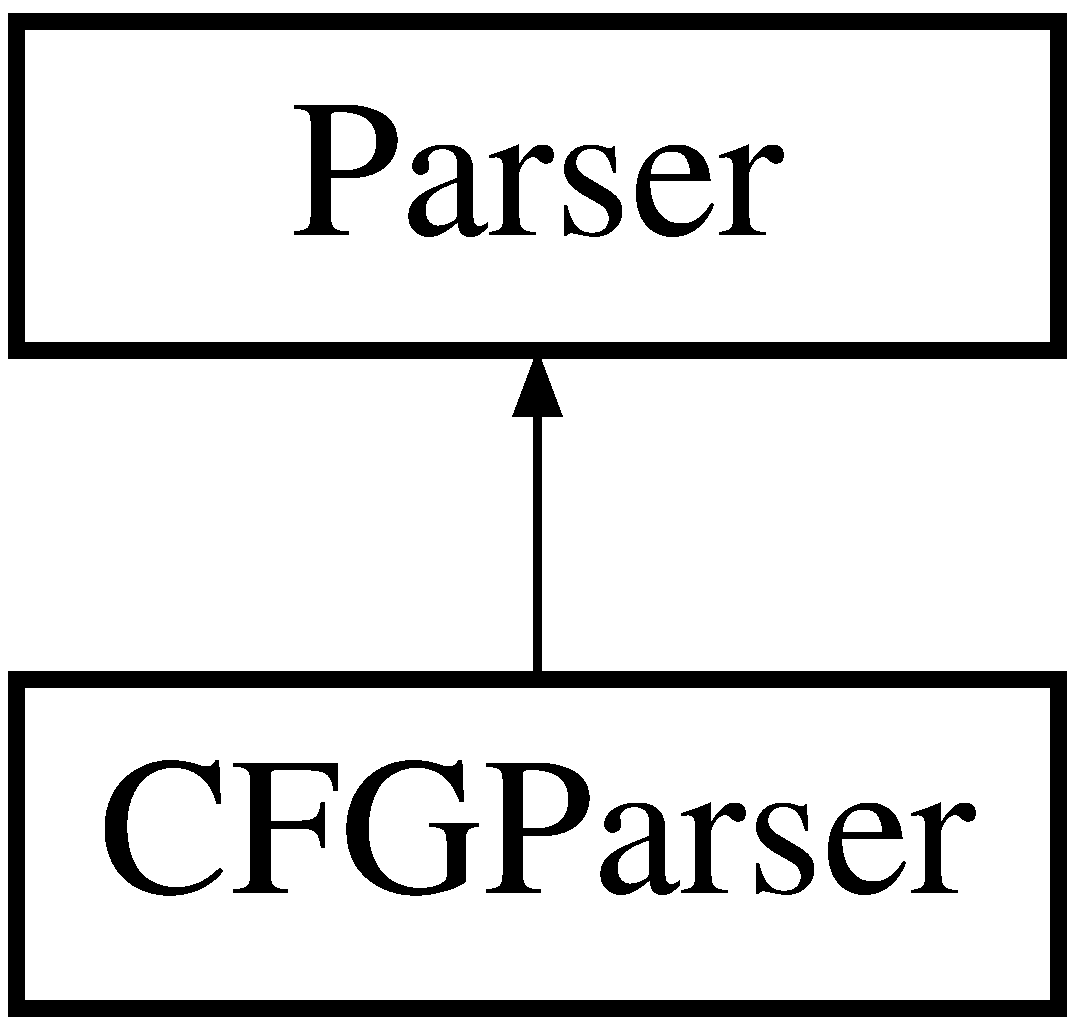
\includegraphics[height=2.000000cm]{da/d24/classCFGParser}
\end{center}
\end{figure}
\subsection*{\-Public \-Member \-Functions}
\begin{DoxyCompactItemize}
\item 
\hyperlink{classCFGParser_ab92c03dd2a8d901fb38b468c97ee879d}{\-C\-F\-G\-Parser} (std\-::string)
\item 
virtual \hyperlink{classCFGParser_a52b7730ad87bfb47fcc100dc6b2756ee}{$\sim$\-C\-F\-G\-Parser} ()
\item 
std\-::vector$<$ std\-::string $>$ \hyperlink{classCFGParser_a91c3dfa2ce514b1066eb4d86af311804}{get\-Variables} () const 
\item 
std\-::vector$<$ std\-::string $>$ \hyperlink{classCFGParser_aef1d5758fe648f2ab93220816bdd9a84}{get\-Terminals} () const 
\item 
std\-::map$<$ std\-::string, \*
std\-::vector$<$ std\-::string $>$ $>$ \hyperlink{classCFGParser_abf6237f25b52dd05009220a8d10c3449}{get\-Rules} () const 
\item 
std\-::string \hyperlink{classCFGParser_af4336389c220320c7d9511fffafddfae}{get\-Start} () const 
\end{DoxyCompactItemize}
\subsection*{\-Private \-Member \-Functions}
\begin{DoxyCompactItemize}
\item 
void \hyperlink{classCFGParser_ad743c15b7790fcd172b8a1ef7ece1473}{parse\-Variables} (\-Ti\-Xml\-Element $\ast$)
\item 
void \hyperlink{classCFGParser_a525642f6ee69770c435e855e0609fa32}{parse\-Terminals} (\-Ti\-Xml\-Element $\ast$)
\item 
void \hyperlink{classCFGParser_a681f962f987adf57ba9ff8b3638fef14}{parse\-Rules} (\-Ti\-Xml\-Element $\ast$)
\item 
void \hyperlink{classCFGParser_a1ca52cabb5cf726a0eb7a2668c3c0a5a}{parse\-Start} (\-Ti\-Xml\-Element $\ast$)
\end{DoxyCompactItemize}
\subsection*{\-Private \-Attributes}
\begin{DoxyCompactItemize}
\item 
std\-::vector$<$ std\-::string $>$ \hyperlink{classCFGParser_a2be700c7eebe5a1a0fd18b88b3074840}{variables}
\item 
std\-::vector$<$ std\-::string $>$ \hyperlink{classCFGParser_a7242b5a22e08de31297dc9bbb367f5bc}{terminals}
\item 
std\-::map$<$ std\-::string, \*
std\-::vector$<$ std\-::string $>$ $>$ \hyperlink{classCFGParser_a9bea0a4314c8f16ac9aaf0a801a42d86}{rules}
\item 
std\-::string \hyperlink{classCFGParser_a3a51f2f7a2f5342ce9016d226869a516}{start\-Symbol}
\end{DoxyCompactItemize}


\subsection{\-Constructor \& \-Destructor \-Documentation}
\hypertarget{classCFGParser_ab92c03dd2a8d901fb38b468c97ee879d}{\index{\-C\-F\-G\-Parser@{\-C\-F\-G\-Parser}!\-C\-F\-G\-Parser@{\-C\-F\-G\-Parser}}
\index{\-C\-F\-G\-Parser@{\-C\-F\-G\-Parser}!CFGParser@{\-C\-F\-G\-Parser}}
\subsubsection[{\-C\-F\-G\-Parser}]{\setlength{\rightskip}{0pt plus 5cm}{\bf \-C\-F\-G\-Parser\-::\-C\-F\-G\-Parser} (
\begin{DoxyParamCaption}
\item[{std\-::string}]{}
\end{DoxyParamCaption}
)}}\label{da/d24/classCFGParser_ab92c03dd2a8d901fb38b468c97ee879d}
\hypertarget{classCFGParser_a52b7730ad87bfb47fcc100dc6b2756ee}{\index{\-C\-F\-G\-Parser@{\-C\-F\-G\-Parser}!$\sim$\-C\-F\-G\-Parser@{$\sim$\-C\-F\-G\-Parser}}
\index{$\sim$\-C\-F\-G\-Parser@{$\sim$\-C\-F\-G\-Parser}!CFGParser@{\-C\-F\-G\-Parser}}
\subsubsection[{$\sim$\-C\-F\-G\-Parser}]{\setlength{\rightskip}{0pt plus 5cm}virtual {\bf \-C\-F\-G\-Parser\-::$\sim$\-C\-F\-G\-Parser} (
\begin{DoxyParamCaption}
{}
\end{DoxyParamCaption}
)\hspace{0.3cm}{\ttfamily  \mbox{[}virtual\mbox{]}}}}\label{da/d24/classCFGParser_a52b7730ad87bfb47fcc100dc6b2756ee}


\subsection{\-Member \-Function \-Documentation}
\hypertarget{classCFGParser_abf6237f25b52dd05009220a8d10c3449}{\index{\-C\-F\-G\-Parser@{\-C\-F\-G\-Parser}!get\-Rules@{get\-Rules}}
\index{get\-Rules@{get\-Rules}!CFGParser@{\-C\-F\-G\-Parser}}
\subsubsection[{get\-Rules}]{\setlength{\rightskip}{0pt plus 5cm}std\-::map$<$std\-::string, std\-::vector$<$std\-::string$>$ $>$ {\bf \-C\-F\-G\-Parser\-::get\-Rules} (
\begin{DoxyParamCaption}
{}
\end{DoxyParamCaption}
) const}}\label{da/d24/classCFGParser_abf6237f25b52dd05009220a8d10c3449}
\hypertarget{classCFGParser_af4336389c220320c7d9511fffafddfae}{\index{\-C\-F\-G\-Parser@{\-C\-F\-G\-Parser}!get\-Start@{get\-Start}}
\index{get\-Start@{get\-Start}!CFGParser@{\-C\-F\-G\-Parser}}
\subsubsection[{get\-Start}]{\setlength{\rightskip}{0pt plus 5cm}std\-::string {\bf \-C\-F\-G\-Parser\-::get\-Start} (
\begin{DoxyParamCaption}
{}
\end{DoxyParamCaption}
) const}}\label{da/d24/classCFGParser_af4336389c220320c7d9511fffafddfae}
\hypertarget{classCFGParser_aef1d5758fe648f2ab93220816bdd9a84}{\index{\-C\-F\-G\-Parser@{\-C\-F\-G\-Parser}!get\-Terminals@{get\-Terminals}}
\index{get\-Terminals@{get\-Terminals}!CFGParser@{\-C\-F\-G\-Parser}}
\subsubsection[{get\-Terminals}]{\setlength{\rightskip}{0pt plus 5cm}std\-::vector$<$std\-::string$>$ {\bf \-C\-F\-G\-Parser\-::get\-Terminals} (
\begin{DoxyParamCaption}
{}
\end{DoxyParamCaption}
) const}}\label{da/d24/classCFGParser_aef1d5758fe648f2ab93220816bdd9a84}
\hypertarget{classCFGParser_a91c3dfa2ce514b1066eb4d86af311804}{\index{\-C\-F\-G\-Parser@{\-C\-F\-G\-Parser}!get\-Variables@{get\-Variables}}
\index{get\-Variables@{get\-Variables}!CFGParser@{\-C\-F\-G\-Parser}}
\subsubsection[{get\-Variables}]{\setlength{\rightskip}{0pt plus 5cm}std\-::vector$<$std\-::string$>$ {\bf \-C\-F\-G\-Parser\-::get\-Variables} (
\begin{DoxyParamCaption}
{}
\end{DoxyParamCaption}
) const}}\label{da/d24/classCFGParser_a91c3dfa2ce514b1066eb4d86af311804}
\hypertarget{classCFGParser_a681f962f987adf57ba9ff8b3638fef14}{\index{\-C\-F\-G\-Parser@{\-C\-F\-G\-Parser}!parse\-Rules@{parse\-Rules}}
\index{parse\-Rules@{parse\-Rules}!CFGParser@{\-C\-F\-G\-Parser}}
\subsubsection[{parse\-Rules}]{\setlength{\rightskip}{0pt plus 5cm}void {\bf \-C\-F\-G\-Parser\-::parse\-Rules} (
\begin{DoxyParamCaption}
\item[{\-Ti\-Xml\-Element $\ast$}]{}
\end{DoxyParamCaption}
)\hspace{0.3cm}{\ttfamily  \mbox{[}private\mbox{]}}}}\label{da/d24/classCFGParser_a681f962f987adf57ba9ff8b3638fef14}
\hypertarget{classCFGParser_a1ca52cabb5cf726a0eb7a2668c3c0a5a}{\index{\-C\-F\-G\-Parser@{\-C\-F\-G\-Parser}!parse\-Start@{parse\-Start}}
\index{parse\-Start@{parse\-Start}!CFGParser@{\-C\-F\-G\-Parser}}
\subsubsection[{parse\-Start}]{\setlength{\rightskip}{0pt plus 5cm}void {\bf \-C\-F\-G\-Parser\-::parse\-Start} (
\begin{DoxyParamCaption}
\item[{\-Ti\-Xml\-Element $\ast$}]{}
\end{DoxyParamCaption}
)\hspace{0.3cm}{\ttfamily  \mbox{[}private\mbox{]}}}}\label{da/d24/classCFGParser_a1ca52cabb5cf726a0eb7a2668c3c0a5a}
\hypertarget{classCFGParser_a525642f6ee69770c435e855e0609fa32}{\index{\-C\-F\-G\-Parser@{\-C\-F\-G\-Parser}!parse\-Terminals@{parse\-Terminals}}
\index{parse\-Terminals@{parse\-Terminals}!CFGParser@{\-C\-F\-G\-Parser}}
\subsubsection[{parse\-Terminals}]{\setlength{\rightskip}{0pt plus 5cm}void {\bf \-C\-F\-G\-Parser\-::parse\-Terminals} (
\begin{DoxyParamCaption}
\item[{\-Ti\-Xml\-Element $\ast$}]{}
\end{DoxyParamCaption}
)\hspace{0.3cm}{\ttfamily  \mbox{[}private\mbox{]}}}}\label{da/d24/classCFGParser_a525642f6ee69770c435e855e0609fa32}
\hypertarget{classCFGParser_ad743c15b7790fcd172b8a1ef7ece1473}{\index{\-C\-F\-G\-Parser@{\-C\-F\-G\-Parser}!parse\-Variables@{parse\-Variables}}
\index{parse\-Variables@{parse\-Variables}!CFGParser@{\-C\-F\-G\-Parser}}
\subsubsection[{parse\-Variables}]{\setlength{\rightskip}{0pt plus 5cm}void {\bf \-C\-F\-G\-Parser\-::parse\-Variables} (
\begin{DoxyParamCaption}
\item[{\-Ti\-Xml\-Element $\ast$}]{}
\end{DoxyParamCaption}
)\hspace{0.3cm}{\ttfamily  \mbox{[}private\mbox{]}}}}\label{da/d24/classCFGParser_ad743c15b7790fcd172b8a1ef7ece1473}


\subsection{\-Member \-Data \-Documentation}
\hypertarget{classCFGParser_a9bea0a4314c8f16ac9aaf0a801a42d86}{\index{\-C\-F\-G\-Parser@{\-C\-F\-G\-Parser}!rules@{rules}}
\index{rules@{rules}!CFGParser@{\-C\-F\-G\-Parser}}
\subsubsection[{rules}]{\setlength{\rightskip}{0pt plus 5cm}std\-::map$<$std\-::string, std\-::vector$<$std\-::string$>$ $>$ {\bf \-C\-F\-G\-Parser\-::rules}\hspace{0.3cm}{\ttfamily  \mbox{[}private\mbox{]}}}}\label{da/d24/classCFGParser_a9bea0a4314c8f16ac9aaf0a801a42d86}
\hypertarget{classCFGParser_a3a51f2f7a2f5342ce9016d226869a516}{\index{\-C\-F\-G\-Parser@{\-C\-F\-G\-Parser}!start\-Symbol@{start\-Symbol}}
\index{start\-Symbol@{start\-Symbol}!CFGParser@{\-C\-F\-G\-Parser}}
\subsubsection[{start\-Symbol}]{\setlength{\rightskip}{0pt plus 5cm}std\-::string {\bf \-C\-F\-G\-Parser\-::start\-Symbol}\hspace{0.3cm}{\ttfamily  \mbox{[}private\mbox{]}}}}\label{da/d24/classCFGParser_a3a51f2f7a2f5342ce9016d226869a516}
\hypertarget{classCFGParser_a7242b5a22e08de31297dc9bbb367f5bc}{\index{\-C\-F\-G\-Parser@{\-C\-F\-G\-Parser}!terminals@{terminals}}
\index{terminals@{terminals}!CFGParser@{\-C\-F\-G\-Parser}}
\subsubsection[{terminals}]{\setlength{\rightskip}{0pt plus 5cm}std\-::vector$<$std\-::string$>$ {\bf \-C\-F\-G\-Parser\-::terminals}\hspace{0.3cm}{\ttfamily  \mbox{[}private\mbox{]}}}}\label{da/d24/classCFGParser_a7242b5a22e08de31297dc9bbb367f5bc}
\hypertarget{classCFGParser_a2be700c7eebe5a1a0fd18b88b3074840}{\index{\-C\-F\-G\-Parser@{\-C\-F\-G\-Parser}!variables@{variables}}
\index{variables@{variables}!CFGParser@{\-C\-F\-G\-Parser}}
\subsubsection[{variables}]{\setlength{\rightskip}{0pt plus 5cm}std\-::vector$<$std\-::string$>$ {\bf \-C\-F\-G\-Parser\-::variables}\hspace{0.3cm}{\ttfamily  \mbox{[}private\mbox{]}}}}\label{da/d24/classCFGParser_a2be700c7eebe5a1a0fd18b88b3074840}


\-The documentation for this class was generated from the following file\-:\begin{DoxyCompactItemize}
\item 
src/\hyperlink{Parser_8h}{\-Parser.\-h}\end{DoxyCompactItemize}

\hypertarget{classCNF__CFG}{\section{\-C\-N\-F\-\_\-\-C\-F\-G \-Class \-Reference}
\label{da/d5c/classCNF__CFG}\index{\-C\-N\-F\-\_\-\-C\-F\-G@{\-C\-N\-F\-\_\-\-C\-F\-G}}
}


{\ttfamily \#include $<$\-C\-F\-G.\-h$>$}

\-Inheritance diagram for \-C\-N\-F\-\_\-\-C\-F\-G\-:\begin{figure}[H]
\begin{center}
\leavevmode
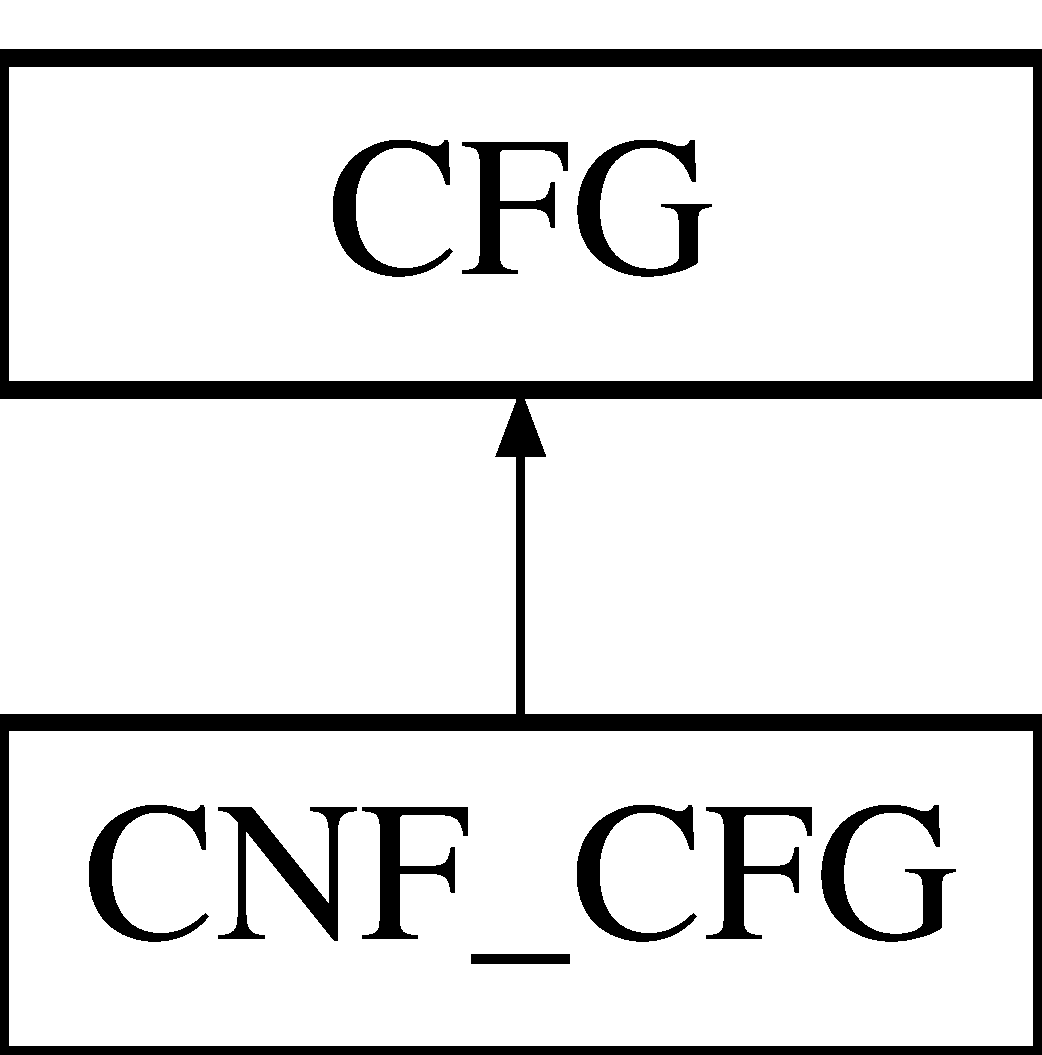
\includegraphics[height=2.000000cm]{da/d5c/classCNF__CFG}
\end{center}
\end{figure}
\subsection*{\-Public \-Member \-Functions}
\begin{DoxyCompactItemize}
\item 
\hyperlink{classCNF__CFG_a3dfe36c6d4b3c69bd4217d71f0fe4746}{\-C\-N\-F\-\_\-\-C\-F\-G} ()
\begin{DoxyCompactList}\small\item\em \-Default constructor. \end{DoxyCompactList}\item 
\hyperlink{classCNF__CFG_a1d22901e8e4c8e25562d4095980537f5}{\-C\-N\-F\-\_\-\-C\-F\-G} (std\-::vector$<$ std\-::string $>$ \&v, std\-::vector$<$ std\-::string $>$ \&t, std\-::map$<$ std\-::string, std\-::vector$<$ std\-::string $>$ $>$ \&r, std\-::string s)
\begin{DoxyCompactList}\small\item\em specified constructor \end{DoxyCompactList}\item 
\hyperlink{classCNF__CFG_aaca2a5cc2e21b1b2e45ddecf3aed65c9}{\-C\-N\-F\-\_\-\-C\-F\-G} (\hyperlink{classCFG}{\-C\-F\-G} \&cfg)
\begin{DoxyCompactList}\small\item\em constructor based on a \hyperlink{classCFG}{\-C\-F\-G} and copy constructor \end{DoxyCompactList}\item 
\hyperlink{classCNF__CFG_a2cde09b5176c556704653475c299952d}{\-C\-N\-F\-\_\-\-C\-F\-G} (std\-::string file)
\begin{DoxyCompactList}\small\item\em constructor with information file \end{DoxyCompactList}\item 
bool \hyperlink{classCNF__CFG_a07436f4035c9fba1cd09761cdec0b02e}{check\-\_\-string} (std\-::string w)
\begin{DoxyCompactList}\small\item\em checks if given string is in the \hyperlink{classCNF__CFG}{\-C\-N\-F\-\_\-\-C\-F\-G} \end{DoxyCompactList}\item 
bool \hyperlink{classCNF__CFG_a418ddb53a7700e331f2791e59d3c1d1f}{already\-\_\-checked} (std\-::string w)
\begin{DoxyCompactList}\small\item\em function used for testing \end{DoxyCompactList}\end{DoxyCompactItemize}
\subsection*{\-Protected \-Member \-Functions}
\begin{DoxyCompactItemize}
\item 
void \hyperlink{classCNF__CFG_a2e368e4718364caf95866d1d692fd49d}{check\-Rules} ()
\begin{DoxyCompactList}\small\item\em map keeps track of all the strings that have already been checked on this \hyperlink{classCFG}{\-C\-F\-G} with the \-C\-Y\-K algorithm \end{DoxyCompactList}\end{DoxyCompactItemize}
\subsection*{\-Protected \-Attributes}
\begin{DoxyCompactItemize}
\item 
\hyperlink{classCYKTable}{\-C\-Y\-K\-Table} \hyperlink{classCNF__CFG_ad8359be441579098a2df2fd979e2f816}{cyk\-\_\-}
\item 
std\-::map$<$ std\-::string, bool $>$ \hyperlink{classCNF__CFG_ac3b39a62d63d5b0fbedf59456355a1f8}{checked}
\begin{DoxyCompactList}\small\item\em used to check if given string is in \hyperlink{classCFG}{\-C\-F\-G} \end{DoxyCompactList}\end{DoxyCompactItemize}


\subsection{\-Constructor \& \-Destructor \-Documentation}
\hypertarget{classCNF__CFG_a3dfe36c6d4b3c69bd4217d71f0fe4746}{\index{\-C\-N\-F\-\_\-\-C\-F\-G@{\-C\-N\-F\-\_\-\-C\-F\-G}!\-C\-N\-F\-\_\-\-C\-F\-G@{\-C\-N\-F\-\_\-\-C\-F\-G}}
\index{\-C\-N\-F\-\_\-\-C\-F\-G@{\-C\-N\-F\-\_\-\-C\-F\-G}!CNF_CFG@{\-C\-N\-F\-\_\-\-C\-F\-G}}
\subsubsection[{\-C\-N\-F\-\_\-\-C\-F\-G}]{\setlength{\rightskip}{0pt plus 5cm}{\bf \-C\-N\-F\-\_\-\-C\-F\-G\-::\-C\-N\-F\-\_\-\-C\-F\-G} (
\begin{DoxyParamCaption}
{}
\end{DoxyParamCaption}
)}}\label{da/d5c/classCNF__CFG_a3dfe36c6d4b3c69bd4217d71f0fe4746}


\-Default constructor. 

\hypertarget{classCNF__CFG_a1d22901e8e4c8e25562d4095980537f5}{\index{\-C\-N\-F\-\_\-\-C\-F\-G@{\-C\-N\-F\-\_\-\-C\-F\-G}!\-C\-N\-F\-\_\-\-C\-F\-G@{\-C\-N\-F\-\_\-\-C\-F\-G}}
\index{\-C\-N\-F\-\_\-\-C\-F\-G@{\-C\-N\-F\-\_\-\-C\-F\-G}!CNF_CFG@{\-C\-N\-F\-\_\-\-C\-F\-G}}
\subsubsection[{\-C\-N\-F\-\_\-\-C\-F\-G}]{\setlength{\rightskip}{0pt plus 5cm}{\bf \-C\-N\-F\-\_\-\-C\-F\-G\-::\-C\-N\-F\-\_\-\-C\-F\-G} (
\begin{DoxyParamCaption}
\item[{std\-::vector$<$ std\-::string $>$ \&}]{v, }
\item[{std\-::vector$<$ std\-::string $>$ \&}]{t, }
\item[{std\-::map$<$ std\-::string, std\-::vector$<$ std\-::string $>$ $>$ \&}]{r, }
\item[{std\-::string}]{s}
\end{DoxyParamCaption}
)}}\label{da/d5c/classCNF__CFG_a1d22901e8e4c8e25562d4095980537f5}


specified constructor 


\begin{DoxyParams}{\-Parameters}
{\em v} & vector with variables \\
\hline
{\em t} & vector with terminals \\
\hline
{\em r} & map with rules of the form $<$\-Variable$>$, vector$<$terminals,\-Variables$>$ \\
\hline
{\em s} & the start symbol for the \hyperlink{classCFG}{\-C\-F\-G} \\
\hline
\end{DoxyParams}
\hypertarget{classCNF__CFG_aaca2a5cc2e21b1b2e45ddecf3aed65c9}{\index{\-C\-N\-F\-\_\-\-C\-F\-G@{\-C\-N\-F\-\_\-\-C\-F\-G}!\-C\-N\-F\-\_\-\-C\-F\-G@{\-C\-N\-F\-\_\-\-C\-F\-G}}
\index{\-C\-N\-F\-\_\-\-C\-F\-G@{\-C\-N\-F\-\_\-\-C\-F\-G}!CNF_CFG@{\-C\-N\-F\-\_\-\-C\-F\-G}}
\subsubsection[{\-C\-N\-F\-\_\-\-C\-F\-G}]{\setlength{\rightskip}{0pt plus 5cm}{\bf \-C\-N\-F\-\_\-\-C\-F\-G\-::\-C\-N\-F\-\_\-\-C\-F\-G} (
\begin{DoxyParamCaption}
\item[{{\bf \-C\-F\-G} \&}]{cfg}
\end{DoxyParamCaption}
)}}\label{da/d5c/classCNF__CFG_aaca2a5cc2e21b1b2e45ddecf3aed65c9}


constructor based on a \hyperlink{classCFG}{\-C\-F\-G} and copy constructor 


\begin{DoxyParams}{\-Parameters}
{\em cfg} & a \hyperlink{classCFG}{\-C\-F\-G} that is in \-C\-N\-F form or a \hyperlink{classCNF__CFG}{\-C\-N\-F\-\_\-\-C\-F\-G} \\
\hline
\end{DoxyParams}
\hypertarget{classCNF__CFG_a2cde09b5176c556704653475c299952d}{\index{\-C\-N\-F\-\_\-\-C\-F\-G@{\-C\-N\-F\-\_\-\-C\-F\-G}!\-C\-N\-F\-\_\-\-C\-F\-G@{\-C\-N\-F\-\_\-\-C\-F\-G}}
\index{\-C\-N\-F\-\_\-\-C\-F\-G@{\-C\-N\-F\-\_\-\-C\-F\-G}!CNF_CFG@{\-C\-N\-F\-\_\-\-C\-F\-G}}
\subsubsection[{\-C\-N\-F\-\_\-\-C\-F\-G}]{\setlength{\rightskip}{0pt plus 5cm}{\bf \-C\-N\-F\-\_\-\-C\-F\-G\-::\-C\-N\-F\-\_\-\-C\-F\-G} (
\begin{DoxyParamCaption}
\item[{std\-::string}]{file}
\end{DoxyParamCaption}
)}}\label{da/d5c/classCNF__CFG_a2cde09b5176c556704653475c299952d}


constructor with information file 



\subsection{\-Member \-Function \-Documentation}
\hypertarget{classCNF__CFG_a418ddb53a7700e331f2791e59d3c1d1f}{\index{\-C\-N\-F\-\_\-\-C\-F\-G@{\-C\-N\-F\-\_\-\-C\-F\-G}!already\-\_\-checked@{already\-\_\-checked}}
\index{already\-\_\-checked@{already\-\_\-checked}!CNF_CFG@{\-C\-N\-F\-\_\-\-C\-F\-G}}
\subsubsection[{already\-\_\-checked}]{\setlength{\rightskip}{0pt plus 5cm}bool {\bf \-C\-N\-F\-\_\-\-C\-F\-G\-::already\-\_\-checked} (
\begin{DoxyParamCaption}
\item[{std\-::string}]{w}
\end{DoxyParamCaption}
)}}\label{da/d5c/classCNF__CFG_a418ddb53a7700e331f2791e59d3c1d1f}


function used for testing 


\begin{DoxyParams}{\-Parameters}
{\em w} & string to check \\
\hline
\end{DoxyParams}
\begin{DoxyReturn}{\-Returns}
bool \-: true if already checked, false if not in language 
\end{DoxyReturn}
\hypertarget{classCNF__CFG_a07436f4035c9fba1cd09761cdec0b02e}{\index{\-C\-N\-F\-\_\-\-C\-F\-G@{\-C\-N\-F\-\_\-\-C\-F\-G}!check\-\_\-string@{check\-\_\-string}}
\index{check\-\_\-string@{check\-\_\-string}!CNF_CFG@{\-C\-N\-F\-\_\-\-C\-F\-G}}
\subsubsection[{check\-\_\-string}]{\setlength{\rightskip}{0pt plus 5cm}bool {\bf \-C\-N\-F\-\_\-\-C\-F\-G\-::check\-\_\-string} (
\begin{DoxyParamCaption}
\item[{std\-::string}]{w}
\end{DoxyParamCaption}
)}}\label{da/d5c/classCNF__CFG_a07436f4035c9fba1cd09761cdec0b02e}


checks if given string is in the \hyperlink{classCNF__CFG}{\-C\-N\-F\-\_\-\-C\-F\-G} 


\begin{DoxyParams}{\-Parameters}
{\em w} & string to check \\
\hline
\end{DoxyParams}
\begin{DoxyReturn}{\-Returns}
bool \-: true if in language, false if not in language 
\end{DoxyReturn}
\hypertarget{classCNF__CFG_a2e368e4718364caf95866d1d692fd49d}{\index{\-C\-N\-F\-\_\-\-C\-F\-G@{\-C\-N\-F\-\_\-\-C\-F\-G}!check\-Rules@{check\-Rules}}
\index{check\-Rules@{check\-Rules}!CNF_CFG@{\-C\-N\-F\-\_\-\-C\-F\-G}}
\subsubsection[{check\-Rules}]{\setlength{\rightskip}{0pt plus 5cm}void {\bf \-C\-N\-F\-\_\-\-C\-F\-G\-::check\-Rules} (
\begin{DoxyParamCaption}
{}
\end{DoxyParamCaption}
)\hspace{0.3cm}{\ttfamily  \mbox{[}protected\mbox{]}}}}\label{da/d5c/classCNF__CFG_a2e368e4718364caf95866d1d692fd49d}


map keeps track of all the strings that have already been checked on this \hyperlink{classCFG}{\-C\-F\-G} with the \-C\-Y\-K algorithm 

checks the rules of the \hyperlink{classCFG}{\-C\-F\-G} to see if they are in \-C\-N\-F form 

\subsection{\-Member \-Data \-Documentation}
\hypertarget{classCNF__CFG_ac3b39a62d63d5b0fbedf59456355a1f8}{\index{\-C\-N\-F\-\_\-\-C\-F\-G@{\-C\-N\-F\-\_\-\-C\-F\-G}!checked@{checked}}
\index{checked@{checked}!CNF_CFG@{\-C\-N\-F\-\_\-\-C\-F\-G}}
\subsubsection[{checked}]{\setlength{\rightskip}{0pt plus 5cm}std\-::map$<$std\-::string, bool$>$ {\bf \-C\-N\-F\-\_\-\-C\-F\-G\-::checked}\hspace{0.3cm}{\ttfamily  \mbox{[}protected\mbox{]}}}}\label{da/d5c/classCNF__CFG_ac3b39a62d63d5b0fbedf59456355a1f8}


used to check if given string is in \hyperlink{classCFG}{\-C\-F\-G} 

\hypertarget{classCNF__CFG_ad8359be441579098a2df2fd979e2f816}{\index{\-C\-N\-F\-\_\-\-C\-F\-G@{\-C\-N\-F\-\_\-\-C\-F\-G}!cyk\-\_\-@{cyk\-\_\-}}
\index{cyk\-\_\-@{cyk\-\_\-}!CNF_CFG@{\-C\-N\-F\-\_\-\-C\-F\-G}}
\subsubsection[{cyk\-\_\-}]{\setlength{\rightskip}{0pt plus 5cm}{\bf \-C\-Y\-K\-Table} {\bf \-C\-N\-F\-\_\-\-C\-F\-G\-::cyk\-\_\-}\hspace{0.3cm}{\ttfamily  \mbox{[}protected\mbox{]}}}}\label{da/d5c/classCNF__CFG_ad8359be441579098a2df2fd979e2f816}


\-The documentation for this class was generated from the following file\-:\begin{DoxyCompactItemize}
\item 
src/\hyperlink{CFG_8h}{\-C\-F\-G.\-h}\end{DoxyCompactItemize}

\hypertarget{classCYKTable}{\section{\-C\-Y\-K\-Table \-Class \-Reference}
\label{d6/dcd/classCYKTable}\index{\-C\-Y\-K\-Table@{\-C\-Y\-K\-Table}}
}


{\ttfamily \#include $<$\-C\-Y\-K\-Table.\-h$>$}

\subsection*{\-Public \-Member \-Functions}
\begin{DoxyCompactItemize}
\item 
\hyperlink{classCYKTable_ac96905a2f347c63cfda59d55fc97d90a}{\-C\-Y\-K\-Table} ()
\begin{DoxyCompactList}\small\item\em default constructor \end{DoxyCompactList}\item 
\hyperlink{classCYKTable_a9bcbd180cfda8d5c47587f67026d89ad}{\-C\-Y\-K\-Table} (std\-::map$<$ std\-::string, std\-::vector$<$ std\-::string $>$ $>$ \&r, std\-::string start\-Symbol)
\begin{DoxyCompactList}\small\item\em specified constructor \end{DoxyCompactList}\item 
\hyperlink{classCYKTable_abd9ea746b2c4ed848819efbf95645cc4}{\-C\-Y\-K\-Table} (std\-::string w, std\-::map$<$ std\-::string, std\-::vector$<$ std\-::string $>$ $>$ \&r, std\-::string st\-S)
\begin{DoxyCompactList}\small\item\em specified constructor (used for testing) \end{DoxyCompactList}\item 
bool \hyperlink{classCYKTable_ac756a60dc99c8557ad5d11e557b30f57}{operator()} (std\-::string w)
\begin{DoxyCompactList}\small\item\em \-A function to check a string. \end{DoxyCompactList}\item 
std\-::vector$<$ std\-::string $>$ \hyperlink{classCYKTable_a9d53e2b07637d13ed72b97b007a09cf4}{at} (unsigned int i, unsigned int j) const 
\begin{DoxyCompactList}\small\item\em a function return vector of variables on given position (in \-C\-Y\-K coordinates) \end{DoxyCompactList}\item 
virtual \hyperlink{classCYKTable_af136b6ce499fe3375cf58a9897f2a855}{$\sim$\-C\-Y\-K\-Table} ()
\item 
std\-::map$<$ std\-::string, \*
std\-::vector$<$ std\-::string $>$ $>$ \hyperlink{classCYKTable_a4f57052001961a166453e5cd224d52e8}{get\-Rules} () const 
\item 
std\-::string \hyperlink{classCYKTable_af2065276b21835ad5ddbdb2d5ac9f90d}{get\-Start\-Symbol} () const 
\item 
\hyperlink{CYKTable_8h_a98fc1757708d007972f5f4640a85323e}{\-Table} \hyperlink{classCYKTable_a8de3508f979280f9b4c4a7b08f68f05a}{get\-Table} () const 
\end{DoxyCompactItemize}
\subsection*{\-Private \-Member \-Functions}
\begin{DoxyCompactItemize}
\item 
void \hyperlink{classCYKTable_a7aaee4d68e79f91fb6ff28b14f63668a}{create\-Table} (std\-::string w)
\begin{DoxyCompactList}\small\item\em \-Function creating table for given string. \end{DoxyCompactList}\item 
void \hyperlink{classCYKTable_a0cef9ae424db0d878c6d22808c1ce37a}{add} (unsigned int i, unsigned int j, std\-::string var)
\begin{DoxyCompactList}\small\item\em \-Function adding a new variable to given position in table. \end{DoxyCompactList}\item 
std\-::vector$<$ std\-::pair\*
$<$ std\-::string, std\-::string $>$ $>$ \hyperlink{classCYKTable_a570a60f85560234161476aa53d526931}{calculate\-Combinations} (unsigned int i, unsigned int k, unsigned int j)
\begin{DoxyCompactList}\small\item\em \-Function calculating all possible pairs of variables between 2 positions in the table. \end{DoxyCompactList}\end{DoxyCompactItemize}
\subsection*{\-Private \-Attributes}
\begin{DoxyCompactItemize}
\item 
\hyperlink{CYKTable_8h_a98fc1757708d007972f5f4640a85323e}{\-Table} \hyperlink{classCYKTable_a847f477bcba128dab98ac8cfa987fd04}{table\-\_\-}
\item 
std\-::map$<$ std\-::string, \*
std\-::vector$<$ std\-::string $>$ $>$ \hyperlink{classCYKTable_a90179858da18c70ad4338af8661ddc8a}{rules\-\_\-}
\begin{DoxyCompactList}\small\item\em \-Table in which the information is stored. \end{DoxyCompactList}\item 
std\-::string \hyperlink{classCYKTable_a789892d83fa60dafe30168633dba22ca}{start\-Symbol\-\_\-}
\end{DoxyCompactItemize}
\subsection*{\-Friends}
\begin{DoxyCompactItemize}
\item 
std\-::ostream \& \hyperlink{classCYKTable_a000e039ebe267650040107125c5247f2}{operator$<$$<$} (std\-::ostream \&out, \hyperlink{classCYKTable}{\-C\-Y\-K\-Table} \&c)
\end{DoxyCompactItemize}


\subsection{\-Constructor \& \-Destructor \-Documentation}
\hypertarget{classCYKTable_ac96905a2f347c63cfda59d55fc97d90a}{\index{\-C\-Y\-K\-Table@{\-C\-Y\-K\-Table}!\-C\-Y\-K\-Table@{\-C\-Y\-K\-Table}}
\index{\-C\-Y\-K\-Table@{\-C\-Y\-K\-Table}!CYKTable@{\-C\-Y\-K\-Table}}
\subsubsection[{\-C\-Y\-K\-Table}]{\setlength{\rightskip}{0pt plus 5cm}{\bf \-C\-Y\-K\-Table\-::\-C\-Y\-K\-Table} (
\begin{DoxyParamCaption}
{}
\end{DoxyParamCaption}
)}}\label{d6/dcd/classCYKTable_ac96905a2f347c63cfda59d55fc97d90a}


default constructor 

\hypertarget{classCYKTable_a9bcbd180cfda8d5c47587f67026d89ad}{\index{\-C\-Y\-K\-Table@{\-C\-Y\-K\-Table}!\-C\-Y\-K\-Table@{\-C\-Y\-K\-Table}}
\index{\-C\-Y\-K\-Table@{\-C\-Y\-K\-Table}!CYKTable@{\-C\-Y\-K\-Table}}
\subsubsection[{\-C\-Y\-K\-Table}]{\setlength{\rightskip}{0pt plus 5cm}{\bf \-C\-Y\-K\-Table\-::\-C\-Y\-K\-Table} (
\begin{DoxyParamCaption}
\item[{std\-::map$<$ std\-::string, std\-::vector$<$ std\-::string $>$ $>$ \&}]{r, }
\item[{std\-::string}]{start\-Symbol}
\end{DoxyParamCaption}
)}}\label{d6/dcd/classCYKTable_a9bcbd180cfda8d5c47587f67026d89ad}


specified constructor 


\begin{DoxyParams}{\-Parameters}
{\em r} & map of rules \\
\hline
{\em start\-Symbol} & the start symbol \\
\hline
\end{DoxyParams}
\hypertarget{classCYKTable_abd9ea746b2c4ed848819efbf95645cc4}{\index{\-C\-Y\-K\-Table@{\-C\-Y\-K\-Table}!\-C\-Y\-K\-Table@{\-C\-Y\-K\-Table}}
\index{\-C\-Y\-K\-Table@{\-C\-Y\-K\-Table}!CYKTable@{\-C\-Y\-K\-Table}}
\subsubsection[{\-C\-Y\-K\-Table}]{\setlength{\rightskip}{0pt plus 5cm}{\bf \-C\-Y\-K\-Table\-::\-C\-Y\-K\-Table} (
\begin{DoxyParamCaption}
\item[{std\-::string}]{w, }
\item[{std\-::map$<$ std\-::string, std\-::vector$<$ std\-::string $>$ $>$ \&}]{r, }
\item[{std\-::string}]{st\-S}
\end{DoxyParamCaption}
)}}\label{d6/dcd/classCYKTable_abd9ea746b2c4ed848819efbf95645cc4}


specified constructor (used for testing) 


\begin{DoxyParams}{\-Parameters}
{\em w} & string that will be checked \\
\hline
{\em r} & map of rules \\
\hline
{\em start\-Symbol} & the start symbol \\
\hline
\end{DoxyParams}
\hypertarget{classCYKTable_af136b6ce499fe3375cf58a9897f2a855}{\index{\-C\-Y\-K\-Table@{\-C\-Y\-K\-Table}!$\sim$\-C\-Y\-K\-Table@{$\sim$\-C\-Y\-K\-Table}}
\index{$\sim$\-C\-Y\-K\-Table@{$\sim$\-C\-Y\-K\-Table}!CYKTable@{\-C\-Y\-K\-Table}}
\subsubsection[{$\sim$\-C\-Y\-K\-Table}]{\setlength{\rightskip}{0pt plus 5cm}virtual {\bf \-C\-Y\-K\-Table\-::$\sim$\-C\-Y\-K\-Table} (
\begin{DoxyParamCaption}
{}
\end{DoxyParamCaption}
)\hspace{0.3cm}{\ttfamily  \mbox{[}virtual\mbox{]}}}}\label{d6/dcd/classCYKTable_af136b6ce499fe3375cf58a9897f2a855}


\subsection{\-Member \-Function \-Documentation}
\hypertarget{classCYKTable_a0cef9ae424db0d878c6d22808c1ce37a}{\index{\-C\-Y\-K\-Table@{\-C\-Y\-K\-Table}!add@{add}}
\index{add@{add}!CYKTable@{\-C\-Y\-K\-Table}}
\subsubsection[{add}]{\setlength{\rightskip}{0pt plus 5cm}void {\bf \-C\-Y\-K\-Table\-::add} (
\begin{DoxyParamCaption}
\item[{unsigned int}]{i, }
\item[{unsigned int}]{j, }
\item[{std\-::string}]{var}
\end{DoxyParamCaption}
)\hspace{0.3cm}{\ttfamily  \mbox{[}private\mbox{]}}}}\label{d6/dcd/classCYKTable_a0cef9ae424db0d878c6d22808c1ce37a}


\-Function adding a new variable to given position in table. 


\begin{DoxyParams}{\-Parameters}
{\em i} & \-Nr of the collumn \\
\hline
{\em j} & \-Nr of row + i \\
\hline
\end{DoxyParams}
\hypertarget{classCYKTable_a9d53e2b07637d13ed72b97b007a09cf4}{\index{\-C\-Y\-K\-Table@{\-C\-Y\-K\-Table}!at@{at}}
\index{at@{at}!CYKTable@{\-C\-Y\-K\-Table}}
\subsubsection[{at}]{\setlength{\rightskip}{0pt plus 5cm}std\-::vector$<$std\-::string$>$ {\bf \-C\-Y\-K\-Table\-::at} (
\begin{DoxyParamCaption}
\item[{unsigned int}]{i, }
\item[{unsigned int}]{j}
\end{DoxyParamCaption}
) const}}\label{d6/dcd/classCYKTable_a9d53e2b07637d13ed72b97b007a09cf4}


a function return vector of variables on given position (in \-C\-Y\-K coordinates) 


\begin{DoxyParams}{\-Parameters}
{\em i} & \-Nr of the collumn \\
\hline
{\em j} & \-Nr of row + i \\
\hline
\end{DoxyParams}
\hypertarget{classCYKTable_a570a60f85560234161476aa53d526931}{\index{\-C\-Y\-K\-Table@{\-C\-Y\-K\-Table}!calculate\-Combinations@{calculate\-Combinations}}
\index{calculate\-Combinations@{calculate\-Combinations}!CYKTable@{\-C\-Y\-K\-Table}}
\subsubsection[{calculate\-Combinations}]{\setlength{\rightskip}{0pt plus 5cm}std\-::vector$<$std\-::pair$<$std\-::string, std\-::string$>$ $>$ {\bf \-C\-Y\-K\-Table\-::calculate\-Combinations} (
\begin{DoxyParamCaption}
\item[{unsigned int}]{i, }
\item[{unsigned int}]{k, }
\item[{unsigned int}]{j}
\end{DoxyParamCaption}
)\hspace{0.3cm}{\ttfamily  \mbox{[}private\mbox{]}}}}\label{d6/dcd/classCYKTable_a570a60f85560234161476aa53d526931}


\-Function calculating all possible pairs of variables between 2 positions in the table. 


\begin{DoxyParams}{\-Parameters}
{\em i} & \-Nr of the collumn for 1st position \\
\hline
{\em k} & \-Nr of row + i for 1st el, \-Nr of collumn for 2nd position \\
\hline
{\em j} & \-Nr of row + k for 2nd position \\
\hline
\end{DoxyParams}
\begin{DoxyReturn}{\-Returns}
\-Vector of all pairs with combinations of variables from the 2 positions 
\end{DoxyReturn}
\hypertarget{classCYKTable_a7aaee4d68e79f91fb6ff28b14f63668a}{\index{\-C\-Y\-K\-Table@{\-C\-Y\-K\-Table}!create\-Table@{create\-Table}}
\index{create\-Table@{create\-Table}!CYKTable@{\-C\-Y\-K\-Table}}
\subsubsection[{create\-Table}]{\setlength{\rightskip}{0pt plus 5cm}void {\bf \-C\-Y\-K\-Table\-::create\-Table} (
\begin{DoxyParamCaption}
\item[{std\-::string}]{w}
\end{DoxyParamCaption}
)\hspace{0.3cm}{\ttfamily  \mbox{[}private\mbox{]}}}}\label{d6/dcd/classCYKTable_a7aaee4d68e79f91fb6ff28b14f63668a}


\-Function creating table for given string. 

\hypertarget{classCYKTable_a4f57052001961a166453e5cd224d52e8}{\index{\-C\-Y\-K\-Table@{\-C\-Y\-K\-Table}!get\-Rules@{get\-Rules}}
\index{get\-Rules@{get\-Rules}!CYKTable@{\-C\-Y\-K\-Table}}
\subsubsection[{get\-Rules}]{\setlength{\rightskip}{0pt plus 5cm}std\-::map$<$std\-::string, std\-::vector$<$std\-::string$>$ $>$ {\bf \-C\-Y\-K\-Table\-::get\-Rules} (
\begin{DoxyParamCaption}
{}
\end{DoxyParamCaption}
) const}}\label{d6/dcd/classCYKTable_a4f57052001961a166453e5cd224d52e8}
\hypertarget{classCYKTable_af2065276b21835ad5ddbdb2d5ac9f90d}{\index{\-C\-Y\-K\-Table@{\-C\-Y\-K\-Table}!get\-Start\-Symbol@{get\-Start\-Symbol}}
\index{get\-Start\-Symbol@{get\-Start\-Symbol}!CYKTable@{\-C\-Y\-K\-Table}}
\subsubsection[{get\-Start\-Symbol}]{\setlength{\rightskip}{0pt plus 5cm}std\-::string {\bf \-C\-Y\-K\-Table\-::get\-Start\-Symbol} (
\begin{DoxyParamCaption}
{}
\end{DoxyParamCaption}
) const}}\label{d6/dcd/classCYKTable_af2065276b21835ad5ddbdb2d5ac9f90d}
\hypertarget{classCYKTable_a8de3508f979280f9b4c4a7b08f68f05a}{\index{\-C\-Y\-K\-Table@{\-C\-Y\-K\-Table}!get\-Table@{get\-Table}}
\index{get\-Table@{get\-Table}!CYKTable@{\-C\-Y\-K\-Table}}
\subsubsection[{get\-Table}]{\setlength{\rightskip}{0pt plus 5cm}{\bf \-Table} {\bf \-C\-Y\-K\-Table\-::get\-Table} (
\begin{DoxyParamCaption}
{}
\end{DoxyParamCaption}
) const}}\label{d6/dcd/classCYKTable_a8de3508f979280f9b4c4a7b08f68f05a}
\hypertarget{classCYKTable_ac756a60dc99c8557ad5d11e557b30f57}{\index{\-C\-Y\-K\-Table@{\-C\-Y\-K\-Table}!operator()@{operator()}}
\index{operator()@{operator()}!CYKTable@{\-C\-Y\-K\-Table}}
\subsubsection[{operator()}]{\setlength{\rightskip}{0pt plus 5cm}bool \-C\-Y\-K\-Table\-::operator() (
\begin{DoxyParamCaption}
\item[{std\-::string}]{w}
\end{DoxyParamCaption}
)}}\label{d6/dcd/classCYKTable_ac756a60dc99c8557ad5d11e557b30f57}


\-A function to check a string. 


\begin{DoxyParams}{\-Parameters}
{\em w} & \-A string with which the table will be constructed \\
\hline
\end{DoxyParams}
\begin{DoxyReturn}{\-Returns}
true if string is in \hyperlink{classCFG}{\-C\-F\-G}, false if not 
\end{DoxyReturn}


\subsection{\-Friends \-And \-Related \-Function \-Documentation}
\hypertarget{classCYKTable_a000e039ebe267650040107125c5247f2}{\index{\-C\-Y\-K\-Table@{\-C\-Y\-K\-Table}!operator$<$$<$@{operator$<$$<$}}
\index{operator$<$$<$@{operator$<$$<$}!CYKTable@{\-C\-Y\-K\-Table}}
\subsubsection[{operator$<$$<$}]{\setlength{\rightskip}{0pt plus 5cm}std\-::ostream\& operator$<$$<$ (
\begin{DoxyParamCaption}
\item[{std\-::ostream \&}]{out, }
\item[{{\bf \-C\-Y\-K\-Table} \&}]{c}
\end{DoxyParamCaption}
)\hspace{0.3cm}{\ttfamily  \mbox{[}friend\mbox{]}}}}\label{d6/dcd/classCYKTable_a000e039ebe267650040107125c5247f2}


\subsection{\-Member \-Data \-Documentation}
\hypertarget{classCYKTable_a90179858da18c70ad4338af8661ddc8a}{\index{\-C\-Y\-K\-Table@{\-C\-Y\-K\-Table}!rules\-\_\-@{rules\-\_\-}}
\index{rules\-\_\-@{rules\-\_\-}!CYKTable@{\-C\-Y\-K\-Table}}
\subsubsection[{rules\-\_\-}]{\setlength{\rightskip}{0pt plus 5cm}std\-::map$<$std\-::string, std\-::vector$<$std\-::string$>$ $>$ {\bf \-C\-Y\-K\-Table\-::rules\-\_\-}\hspace{0.3cm}{\ttfamily  \mbox{[}private\mbox{]}}}}\label{d6/dcd/classCYKTable_a90179858da18c70ad4338af8661ddc8a}


\-Table in which the information is stored. 

\hypertarget{classCYKTable_a789892d83fa60dafe30168633dba22ca}{\index{\-C\-Y\-K\-Table@{\-C\-Y\-K\-Table}!start\-Symbol\-\_\-@{start\-Symbol\-\_\-}}
\index{start\-Symbol\-\_\-@{start\-Symbol\-\_\-}!CYKTable@{\-C\-Y\-K\-Table}}
\subsubsection[{start\-Symbol\-\_\-}]{\setlength{\rightskip}{0pt plus 5cm}std\-::string {\bf \-C\-Y\-K\-Table\-::start\-Symbol\-\_\-}\hspace{0.3cm}{\ttfamily  \mbox{[}private\mbox{]}}}}\label{d6/dcd/classCYKTable_a789892d83fa60dafe30168633dba22ca}
\hypertarget{classCYKTable_a847f477bcba128dab98ac8cfa987fd04}{\index{\-C\-Y\-K\-Table@{\-C\-Y\-K\-Table}!table\-\_\-@{table\-\_\-}}
\index{table\-\_\-@{table\-\_\-}!CYKTable@{\-C\-Y\-K\-Table}}
\subsubsection[{table\-\_\-}]{\setlength{\rightskip}{0pt plus 5cm}{\bf \-Table} {\bf \-C\-Y\-K\-Table\-::table\-\_\-}\hspace{0.3cm}{\ttfamily  \mbox{[}private\mbox{]}}}}\label{d6/dcd/classCYKTable_a847f477bcba128dab98ac8cfa987fd04}


\-The documentation for this class was generated from the following file\-:\begin{DoxyCompactItemize}
\item 
src/\hyperlink{CYKTable_8h}{\-C\-Y\-K\-Table.\-h}\end{DoxyCompactItemize}

\hypertarget{classException}{\section{Exception Class Reference}
\label{classException}\index{Exception@{Exception}}
}


{\ttfamily \#include $<$Exception.\-h$>$}

Inheritance diagram for Exception\-:\begin{figure}[H]
\begin{center}
\leavevmode
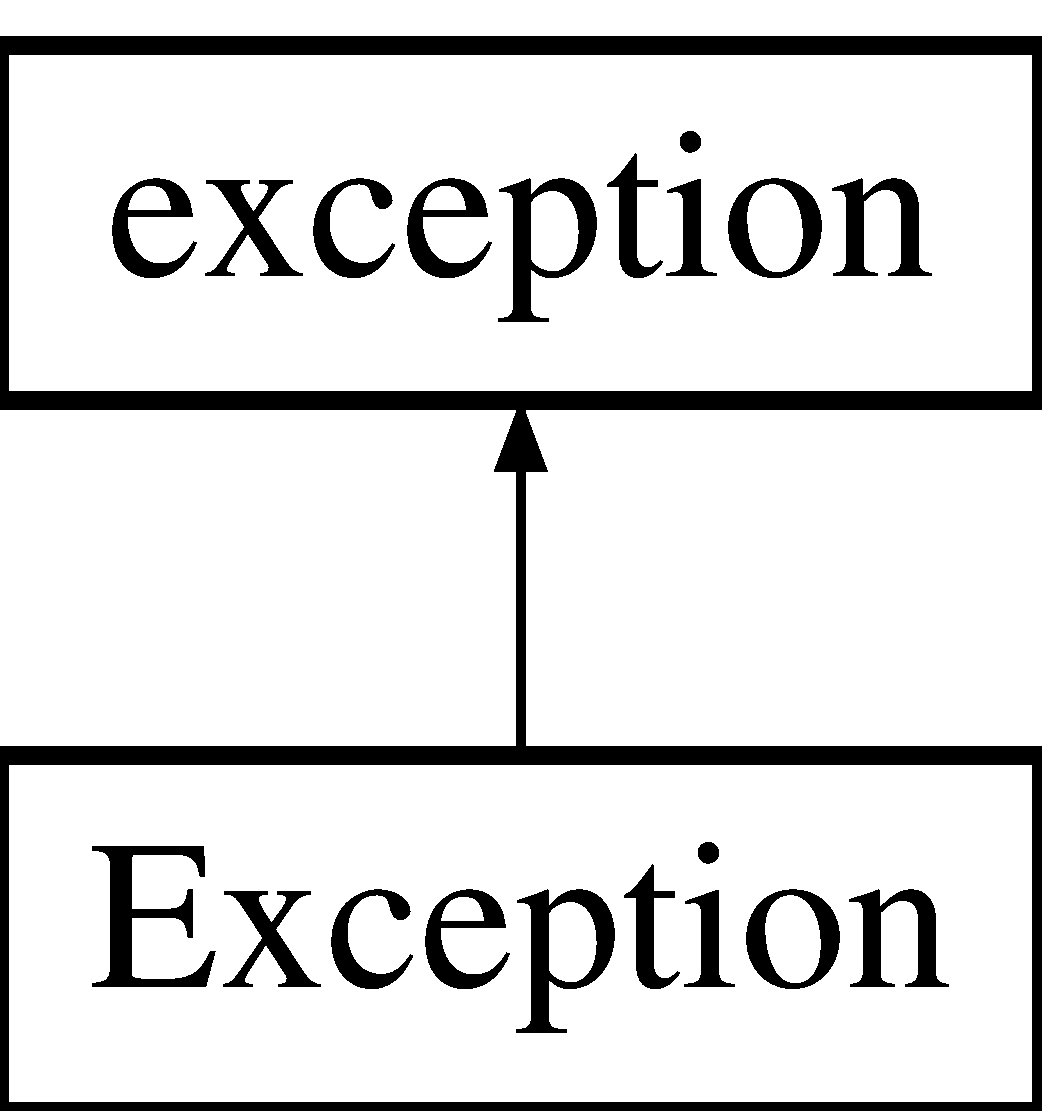
\includegraphics[height=2.000000cm]{d4/d67/classException}
\end{center}
\end{figure}
\subsection*{Public Member Functions}
\begin{DoxyCompactItemize}
\item 
\hyperlink{classException_a1b78336bb26edf8e784783cc150c5801}{Exception} ()
\item 
\hyperlink{classException_a63246c90246de105568d97b0164954d8}{Exception} (std\-::string)
\item 
std\-::string \hyperlink{classException_ae40b22a7b2471b142d861bc33b51a820}{what} ()
\item 
\hyperlink{classException_a6b214cd8627d0968bdeebc1fbb9556b8}{$\sim$\-Exception} ()  throw ()
\end{DoxyCompactItemize}
\subsection*{Private Attributes}
\begin{DoxyCompactItemize}
\item 
std\-::string \hyperlink{classException_a404e79b557f64d95acfb5dccbb864860}{text\-\_\-}
\end{DoxyCompactItemize}


\subsection{Constructor \& Destructor Documentation}
\hypertarget{classException_a1b78336bb26edf8e784783cc150c5801}{\index{Exception@{Exception}!Exception@{Exception}}
\index{Exception@{Exception}!Exception@{Exception}}
\subsubsection[{Exception}]{\setlength{\rightskip}{0pt plus 5cm}Exception\-::\-Exception (
\begin{DoxyParamCaption}
{}
\end{DoxyParamCaption}
)}}\label{classException_a1b78336bb26edf8e784783cc150c5801}
\hypertarget{classException_a63246c90246de105568d97b0164954d8}{\index{Exception@{Exception}!Exception@{Exception}}
\index{Exception@{Exception}!Exception@{Exception}}
\subsubsection[{Exception}]{\setlength{\rightskip}{0pt plus 5cm}Exception\-::\-Exception (
\begin{DoxyParamCaption}
\item[{std\-::string}]{}
\end{DoxyParamCaption}
)}}\label{classException_a63246c90246de105568d97b0164954d8}
\hypertarget{classException_a6b214cd8627d0968bdeebc1fbb9556b8}{\index{Exception@{Exception}!$\sim$\-Exception@{$\sim$\-Exception}}
\index{$\sim$\-Exception@{$\sim$\-Exception}!Exception@{Exception}}
\subsubsection[{$\sim$\-Exception}]{\setlength{\rightskip}{0pt plus 5cm}Exception\-::$\sim$\-Exception (
\begin{DoxyParamCaption}
{}
\end{DoxyParamCaption}
) throw  ) }}\label{classException_a6b214cd8627d0968bdeebc1fbb9556b8}


\subsection{Member Function Documentation}
\hypertarget{classException_ae40b22a7b2471b142d861bc33b51a820}{\index{Exception@{Exception}!what@{what}}
\index{what@{what}!Exception@{Exception}}
\subsubsection[{what}]{\setlength{\rightskip}{0pt plus 5cm}std\-::string Exception\-::what (
\begin{DoxyParamCaption}
{}
\end{DoxyParamCaption}
)}}\label{classException_ae40b22a7b2471b142d861bc33b51a820}


\subsection{Member Data Documentation}
\hypertarget{classException_a404e79b557f64d95acfb5dccbb864860}{\index{Exception@{Exception}!text\-\_\-@{text\-\_\-}}
\index{text\-\_\-@{text\-\_\-}!Exception@{Exception}}
\subsubsection[{text\-\_\-}]{\setlength{\rightskip}{0pt plus 5cm}std\-::string Exception\-::text\-\_\-\hspace{0.3cm}{\ttfamily [private]}}}\label{classException_a404e79b557f64d95acfb5dccbb864860}


The documentation for this class was generated from the following file\-:\begin{DoxyCompactItemize}
\item 
src/\hyperlink{Exception_8h}{Exception.\-h}\end{DoxyCompactItemize}

\hypertarget{classLRParser}{\section{L\-R\-Parser Class Reference}
\label{classLRParser}\index{L\-R\-Parser@{L\-R\-Parser}}
}


{\ttfamily \#include $<$L\-R\-Parser.\-h$>$}

Inheritance diagram for L\-R\-Parser\-:\begin{figure}[H]
\begin{center}
\leavevmode
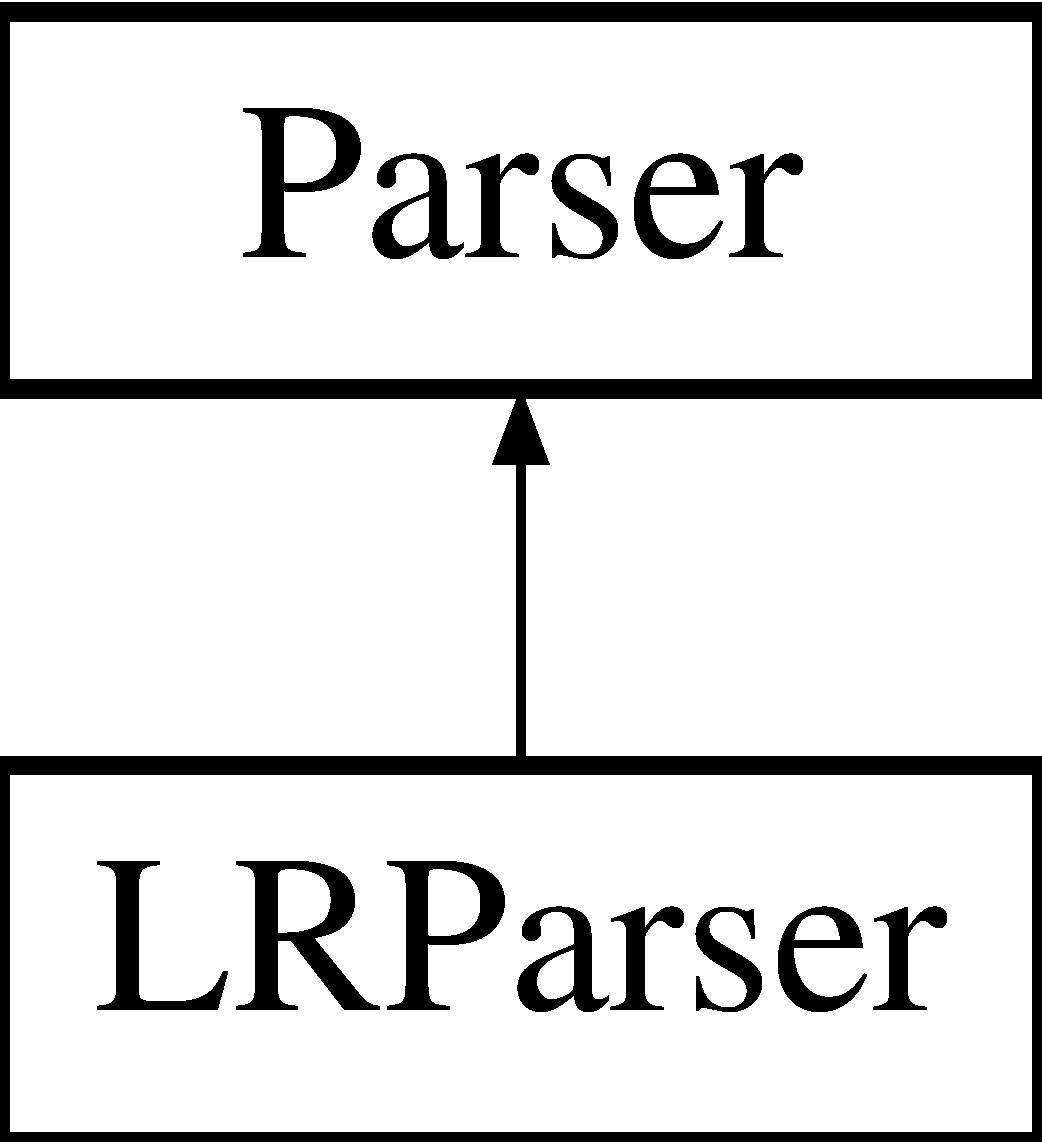
\includegraphics[height=2.000000cm]{d6/de9/classLRParser}
\end{center}
\end{figure}
\subsection*{Public Member Functions}
\begin{DoxyCompactItemize}
\item 
\hyperlink{classLRParser_adf2fe54095f02900d06389007a1e5f53}{L\-R\-Parser} ()
\begin{DoxyCompactList}\small\item\em Default constructor for \hyperlink{classLRParser}{L\-R\-Parser}. This won't be able to do anything as it has no parse table. \end{DoxyCompactList}\item 
\hyperlink{classLRParser_abee4e9919e49f66051167487fb467601}{L\-R\-Parser} (\hyperlink{classCFG}{C\-F\-G})
\begin{DoxyCompactList}\small\item\em The \hyperlink{classCFG}{C\-F\-G} defines the C\-F\-L. The parse table will be generated from this grammar. \end{DoxyCompactList}\item 
\hyperlink{classLRParser_a52727298bd32f6b4ac91d2e1351ffe49}{L\-R\-Parser} (\hyperlink{classParseTable}{Parse\-Table})
\begin{DoxyCompactList}\small\item\em The parameter \hyperlink{classParseTable}{Parse\-Table} will be directly used. \end{DoxyCompactList}\item 
bool \hyperlink{classLRParser_a0657ab1ec68beb8fce3756f7204079b4}{parse} (std\-::string)
\begin{DoxyCompactList}\small\item\em Parses the given input string and returns true if it is valid, false if it is invalid. \end{DoxyCompactList}\item 
std\-::stack$<$ std\-::string $>$ \hyperlink{classLRParser_ac832f117eb1ff5f21d9ed0a7426937a5}{get\-Stack} ()
\item 
unsigned int \hyperlink{classLRParser_a817415c2083c538a0380eace8ec4df5e}{get\-Counter} ()
\item 
virtual \hyperlink{classLRParser_a85b1487a331f1a617ee74965264fcf8f}{$\sim$\-L\-R\-Parser} ()
\end{DoxyCompactItemize}
\subsection*{Protected Member Functions}
\begin{DoxyCompactItemize}
\item 
std\-::pair$<$ \hyperlink{ParseTable_8h_a81d4868b129e5f45325894085a36a8a5}{E\-Action}, std\-::string $>$ \hyperlink{classLRParser_a3bd6bff5276c4ee9b592a14e31e789b3}{process\-Symbol} ()
\begin{DoxyCompactList}\small\item\em Counter used to track at what character of our input we're at. \end{DoxyCompactList}\item 
bool \hyperlink{classLRParser_aa2a11e0af8cbc1bb23b522f1a2ca87e5}{perform\-Action} (std\-::pair$<$ \hyperlink{ParseTable_8h_a81d4868b129e5f45325894085a36a8a5}{E\-Action}, std\-::string $>$)
\begin{DoxyCompactList}\small\item\em Performs action. If this evaluates to true the function it means that input\-\_\- was valid. \end{DoxyCompactList}\item 
bool \hyperlink{classLRParser_ab355d762edcb2c7da1f30728d08b43a1}{handle\-Reduction} (std\-::string)
\begin{DoxyCompactList}\small\item\em Handles the reduction action. \end{DoxyCompactList}\end{DoxyCompactItemize}
\subsection*{Protected Attributes}
\begin{DoxyCompactItemize}
\item 
\hyperlink{classParseTable}{Parse\-Table} \hyperlink{classLRParser_a111f4dd04eb42896c7c31bd1a255a58b}{p\-\_\-table\-\_\-}
\item 
std\-::stack$<$ std\-::string $>$ \hyperlink{classLRParser_a98af41152079cb4f2fe7f280629cf18c}{stack\-\_\-}
\item 
std\-::string \hyperlink{classLRParser_a8dc38b1c7c3a3aa80abbd48ee2364319}{input\-\_\-}
\item 
unsigned int \hyperlink{classLRParser_acd3eab842429e90bd7dc0433274e0a37}{counter\-\_\-}
\end{DoxyCompactItemize}
\subsection*{Friends}
\begin{DoxyCompactItemize}
\item 
std\-::ostream \& \hyperlink{classLRParser_a9f53bcd94244f30103c9756aabf51d38}{operator$<$$<$} (std\-::ostream \&, \hyperlink{classLRParser}{L\-R\-Parser} \&)
\begin{DoxyCompactList}\small\item\em Overloaded output operator\-: shows the stack contents;. \end{DoxyCompactList}\end{DoxyCompactItemize}


\subsection{Constructor \& Destructor Documentation}
\hypertarget{classLRParser_adf2fe54095f02900d06389007a1e5f53}{\index{L\-R\-Parser@{L\-R\-Parser}!L\-R\-Parser@{L\-R\-Parser}}
\index{L\-R\-Parser@{L\-R\-Parser}!LRParser@{L\-R\-Parser}}
\subsubsection[{L\-R\-Parser}]{\setlength{\rightskip}{0pt plus 5cm}L\-R\-Parser\-::\-L\-R\-Parser (
\begin{DoxyParamCaption}
{}
\end{DoxyParamCaption}
)}}\label{classLRParser_adf2fe54095f02900d06389007a1e5f53}


Default constructor for \hyperlink{classLRParser}{L\-R\-Parser}. This won't be able to do anything as it has no parse table. 

\hypertarget{classLRParser_abee4e9919e49f66051167487fb467601}{\index{L\-R\-Parser@{L\-R\-Parser}!L\-R\-Parser@{L\-R\-Parser}}
\index{L\-R\-Parser@{L\-R\-Parser}!LRParser@{L\-R\-Parser}}
\subsubsection[{L\-R\-Parser}]{\setlength{\rightskip}{0pt plus 5cm}L\-R\-Parser\-::\-L\-R\-Parser (
\begin{DoxyParamCaption}
\item[{{\bf C\-F\-G}}]{}
\end{DoxyParamCaption}
)}}\label{classLRParser_abee4e9919e49f66051167487fb467601}


The \hyperlink{classCFG}{C\-F\-G} defines the C\-F\-L. The parse table will be generated from this grammar. 


\begin{DoxyParams}{Parameters}
{\em grammar} & grammar for our \hyperlink{classLRParser}{L\-R\-Parser}. \\
\hline
\end{DoxyParams}
\hypertarget{classLRParser_a52727298bd32f6b4ac91d2e1351ffe49}{\index{L\-R\-Parser@{L\-R\-Parser}!L\-R\-Parser@{L\-R\-Parser}}
\index{L\-R\-Parser@{L\-R\-Parser}!LRParser@{L\-R\-Parser}}
\subsubsection[{L\-R\-Parser}]{\setlength{\rightskip}{0pt plus 5cm}L\-R\-Parser\-::\-L\-R\-Parser (
\begin{DoxyParamCaption}
\item[{{\bf Parse\-Table}}]{}
\end{DoxyParamCaption}
)}}\label{classLRParser_a52727298bd32f6b4ac91d2e1351ffe49}


The parameter \hyperlink{classParseTable}{Parse\-Table} will be directly used. 


\begin{DoxyParams}{Parameters}
{\em pt} & \hyperlink{classParseTable}{Parse\-Table} for our \hyperlink{classLRParser}{L\-R\-Parser}. \\
\hline
\end{DoxyParams}
\hypertarget{classLRParser_a85b1487a331f1a617ee74965264fcf8f}{\index{L\-R\-Parser@{L\-R\-Parser}!$\sim$\-L\-R\-Parser@{$\sim$\-L\-R\-Parser}}
\index{$\sim$\-L\-R\-Parser@{$\sim$\-L\-R\-Parser}!LRParser@{L\-R\-Parser}}
\subsubsection[{$\sim$\-L\-R\-Parser}]{\setlength{\rightskip}{0pt plus 5cm}virtual L\-R\-Parser\-::$\sim$\-L\-R\-Parser (
\begin{DoxyParamCaption}
{}
\end{DoxyParamCaption}
)\hspace{0.3cm}{\ttfamily [virtual]}}}\label{classLRParser_a85b1487a331f1a617ee74965264fcf8f}


\subsection{Member Function Documentation}
\hypertarget{classLRParser_a817415c2083c538a0380eace8ec4df5e}{\index{L\-R\-Parser@{L\-R\-Parser}!get\-Counter@{get\-Counter}}
\index{get\-Counter@{get\-Counter}!LRParser@{L\-R\-Parser}}
\subsubsection[{get\-Counter}]{\setlength{\rightskip}{0pt plus 5cm}unsigned int L\-R\-Parser\-::get\-Counter (
\begin{DoxyParamCaption}
{}
\end{DoxyParamCaption}
)}}\label{classLRParser_a817415c2083c538a0380eace8ec4df5e}
\hypertarget{classLRParser_ac832f117eb1ff5f21d9ed0a7426937a5}{\index{L\-R\-Parser@{L\-R\-Parser}!get\-Stack@{get\-Stack}}
\index{get\-Stack@{get\-Stack}!LRParser@{L\-R\-Parser}}
\subsubsection[{get\-Stack}]{\setlength{\rightskip}{0pt plus 5cm}std\-::stack$<$std\-::string$>$ L\-R\-Parser\-::get\-Stack (
\begin{DoxyParamCaption}
{}
\end{DoxyParamCaption}
)}}\label{classLRParser_ac832f117eb1ff5f21d9ed0a7426937a5}
\hypertarget{classLRParser_ab355d762edcb2c7da1f30728d08b43a1}{\index{L\-R\-Parser@{L\-R\-Parser}!handle\-Reduction@{handle\-Reduction}}
\index{handle\-Reduction@{handle\-Reduction}!LRParser@{L\-R\-Parser}}
\subsubsection[{handle\-Reduction}]{\setlength{\rightskip}{0pt plus 5cm}bool L\-R\-Parser\-::handle\-Reduction (
\begin{DoxyParamCaption}
\item[{std\-::string}]{}
\end{DoxyParamCaption}
)\hspace{0.3cm}{\ttfamily [protected]}}}\label{classLRParser_ab355d762edcb2c7da1f30728d08b43a1}


Handles the reduction action. 


\begin{DoxyParams}{Parameters}
{\em input} & is a rule that will be applied from body to head. \\
\hline
\end{DoxyParams}
\hypertarget{classLRParser_a0657ab1ec68beb8fce3756f7204079b4}{\index{L\-R\-Parser@{L\-R\-Parser}!parse@{parse}}
\index{parse@{parse}!LRParser@{L\-R\-Parser}}
\subsubsection[{parse}]{\setlength{\rightskip}{0pt plus 5cm}bool L\-R\-Parser\-::parse (
\begin{DoxyParamCaption}
\item[{std\-::string}]{}
\end{DoxyParamCaption}
)}}\label{classLRParser_a0657ab1ec68beb8fce3756f7204079b4}


Parses the given input string and returns true if it is valid, false if it is invalid. 


\begin{DoxyParams}{Parameters}
{\em input} & input string that will be tested. \\
\hline
\end{DoxyParams}
\hypertarget{classLRParser_aa2a11e0af8cbc1bb23b522f1a2ca87e5}{\index{L\-R\-Parser@{L\-R\-Parser}!perform\-Action@{perform\-Action}}
\index{perform\-Action@{perform\-Action}!LRParser@{L\-R\-Parser}}
\subsubsection[{perform\-Action}]{\setlength{\rightskip}{0pt plus 5cm}bool L\-R\-Parser\-::perform\-Action (
\begin{DoxyParamCaption}
\item[{std\-::pair$<$ {\bf E\-Action}, std\-::string $>$}]{}
\end{DoxyParamCaption}
)\hspace{0.3cm}{\ttfamily [protected]}}}\label{classLRParser_aa2a11e0af8cbc1bb23b522f1a2ca87e5}


Performs action. If this evaluates to true the function it means that input\-\_\- was valid. 


\begin{DoxyParams}{Parameters}
{\em action} & which will be executed. \\
\hline
\end{DoxyParams}
\hypertarget{classLRParser_a3bd6bff5276c4ee9b592a14e31e789b3}{\index{L\-R\-Parser@{L\-R\-Parser}!process\-Symbol@{process\-Symbol}}
\index{process\-Symbol@{process\-Symbol}!LRParser@{L\-R\-Parser}}
\subsubsection[{process\-Symbol}]{\setlength{\rightskip}{0pt plus 5cm}std\-::pair$<${\bf E\-Action}, std\-::string$>$ L\-R\-Parser\-::process\-Symbol (
\begin{DoxyParamCaption}
{}
\end{DoxyParamCaption}
)\hspace{0.3cm}{\ttfamily [protected]}}}\label{classLRParser_a3bd6bff5276c4ee9b592a14e31e789b3}


Counter used to track at what character of our input we're at. 

Reads a symbol from the input and returns what to do. (from parsetable) Also pushes the read symbol on the stack. \begin{DoxyReturn}{Returns}
a pair of what to do (E\-Action) and possible data needed for the action (string). 
\end{DoxyReturn}


\subsection{Friends And Related Function Documentation}
\hypertarget{classLRParser_a9f53bcd94244f30103c9756aabf51d38}{\index{L\-R\-Parser@{L\-R\-Parser}!operator$<$$<$@{operator$<$$<$}}
\index{operator$<$$<$@{operator$<$$<$}!LRParser@{L\-R\-Parser}}
\subsubsection[{operator$<$$<$}]{\setlength{\rightskip}{0pt plus 5cm}std\-::ostream\& operator$<$$<$ (
\begin{DoxyParamCaption}
\item[{std\-::ostream \&}]{, }
\item[{{\bf L\-R\-Parser} \&}]{}
\end{DoxyParamCaption}
)\hspace{0.3cm}{\ttfamily [friend]}}}\label{classLRParser_a9f53bcd94244f30103c9756aabf51d38}


Overloaded output operator\-: shows the stack contents;. 



\subsection{Member Data Documentation}
\hypertarget{classLRParser_acd3eab842429e90bd7dc0433274e0a37}{\index{L\-R\-Parser@{L\-R\-Parser}!counter\-\_\-@{counter\-\_\-}}
\index{counter\-\_\-@{counter\-\_\-}!LRParser@{L\-R\-Parser}}
\subsubsection[{counter\-\_\-}]{\setlength{\rightskip}{0pt plus 5cm}unsigned int L\-R\-Parser\-::counter\-\_\-\hspace{0.3cm}{\ttfamily [protected]}}}\label{classLRParser_acd3eab842429e90bd7dc0433274e0a37}
\hypertarget{classLRParser_a8dc38b1c7c3a3aa80abbd48ee2364319}{\index{L\-R\-Parser@{L\-R\-Parser}!input\-\_\-@{input\-\_\-}}
\index{input\-\_\-@{input\-\_\-}!LRParser@{L\-R\-Parser}}
\subsubsection[{input\-\_\-}]{\setlength{\rightskip}{0pt plus 5cm}std\-::string L\-R\-Parser\-::input\-\_\-\hspace{0.3cm}{\ttfamily [protected]}}}\label{classLRParser_a8dc38b1c7c3a3aa80abbd48ee2364319}
\hypertarget{classLRParser_a111f4dd04eb42896c7c31bd1a255a58b}{\index{L\-R\-Parser@{L\-R\-Parser}!p\-\_\-table\-\_\-@{p\-\_\-table\-\_\-}}
\index{p\-\_\-table\-\_\-@{p\-\_\-table\-\_\-}!LRParser@{L\-R\-Parser}}
\subsubsection[{p\-\_\-table\-\_\-}]{\setlength{\rightskip}{0pt plus 5cm}{\bf Parse\-Table} L\-R\-Parser\-::p\-\_\-table\-\_\-\hspace{0.3cm}{\ttfamily [protected]}}}\label{classLRParser_a111f4dd04eb42896c7c31bd1a255a58b}
\hypertarget{classLRParser_a98af41152079cb4f2fe7f280629cf18c}{\index{L\-R\-Parser@{L\-R\-Parser}!stack\-\_\-@{stack\-\_\-}}
\index{stack\-\_\-@{stack\-\_\-}!LRParser@{L\-R\-Parser}}
\subsubsection[{stack\-\_\-}]{\setlength{\rightskip}{0pt plus 5cm}std\-::stack$<$std\-::string$>$ L\-R\-Parser\-::stack\-\_\-\hspace{0.3cm}{\ttfamily [protected]}}}\label{classLRParser_a98af41152079cb4f2fe7f280629cf18c}


The documentation for this class was generated from the following file\-:\begin{DoxyCompactItemize}
\item 
src/\hyperlink{LRParser_8h}{L\-R\-Parser.\-h}\end{DoxyCompactItemize}

\hypertarget{classParser}{\section{\-Parser \-Class \-Reference}
\label{d0/d40/classParser}\index{\-Parser@{\-Parser}}
}


{\ttfamily \#include $<$\-Parser.\-h$>$}

\-Inheritance diagram for \-Parser\-:\begin{figure}[H]
\begin{center}
\leavevmode
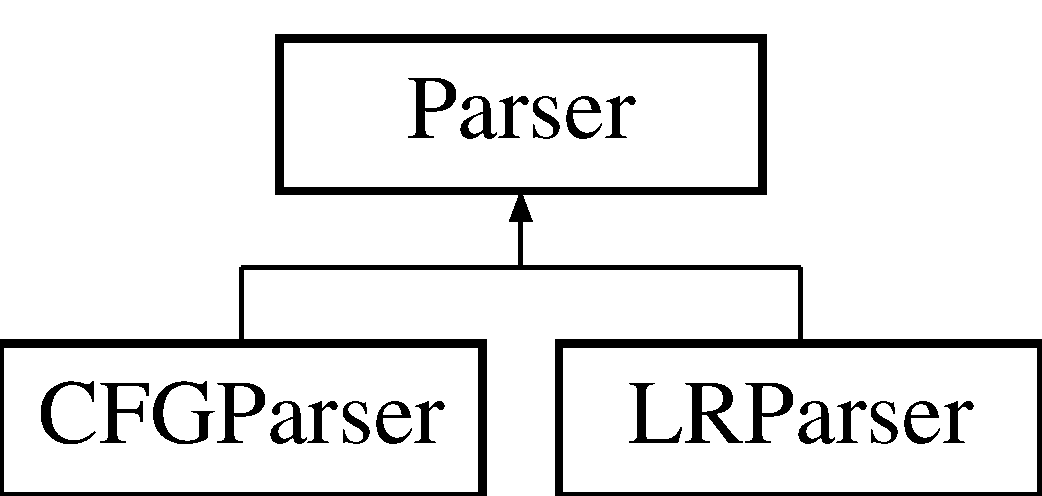
\includegraphics[height=2.000000cm]{d0/d40/classParser}
\end{center}
\end{figure}
\subsection*{\-Public \-Member \-Functions}
\begin{DoxyCompactItemize}
\item 
\hyperlink{classParser_a12234f6cd36b61af4b50c94a179422c1}{\-Parser} ()
\item 
virtual \hyperlink{classParser_ad576b92b9cc324f6f41b0269a9a1a546}{$\sim$\-Parser} ()
\end{DoxyCompactItemize}


\subsection{\-Constructor \& \-Destructor \-Documentation}
\hypertarget{classParser_a12234f6cd36b61af4b50c94a179422c1}{\index{\-Parser@{\-Parser}!\-Parser@{\-Parser}}
\index{\-Parser@{\-Parser}!Parser@{\-Parser}}
\subsubsection[{\-Parser}]{\setlength{\rightskip}{0pt plus 5cm}{\bf \-Parser\-::\-Parser} (
\begin{DoxyParamCaption}
{}
\end{DoxyParamCaption}
)}}\label{d0/d40/classParser_a12234f6cd36b61af4b50c94a179422c1}
\hypertarget{classParser_ad576b92b9cc324f6f41b0269a9a1a546}{\index{\-Parser@{\-Parser}!$\sim$\-Parser@{$\sim$\-Parser}}
\index{$\sim$\-Parser@{$\sim$\-Parser}!Parser@{\-Parser}}
\subsubsection[{$\sim$\-Parser}]{\setlength{\rightskip}{0pt plus 5cm}virtual {\bf \-Parser\-::$\sim$\-Parser} (
\begin{DoxyParamCaption}
{}
\end{DoxyParamCaption}
)\hspace{0.3cm}{\ttfamily  \mbox{[}virtual\mbox{]}}}}\label{d0/d40/classParser_ad576b92b9cc324f6f41b0269a9a1a546}


\-The documentation for this class was generated from the following file\-:\begin{DoxyCompactItemize}
\item 
src/\hyperlink{Parser_8h}{\-Parser.\-h}\end{DoxyCompactItemize}

\hypertarget{classParseTable}{\section{\-Parse\-Table \-Class \-Reference}
\label{d9/da1/classParseTable}\index{\-Parse\-Table@{\-Parse\-Table}}
}


{\ttfamily \#include $<$\-Parse\-Table.\-h$>$}

\subsection*{\-Public \-Member \-Functions}
\begin{DoxyCompactItemize}
\item 
\hyperlink{classParseTable_acacf41ffea967138a7eb200a1d03c0bf}{\-Parse\-Table} ()
\begin{DoxyCompactList}\small\item\em \-Default constructor. \-Our \hyperlink{classParseTable}{\-Parse\-Table} will be empty as it has no \hyperlink{classCFG}{\-C\-F\-G}. \end{DoxyCompactList}\item 
\hyperlink{classParseTable_a71107a2b7d2b83142a31d08d9e960fee}{\-Parse\-Table} (\hyperlink{classCFG}{\-C\-F\-G})
\begin{DoxyCompactList}\small\item\em \-Our \hyperlink{classParseTable}{\-Parse\-Table} will be constructed using the \hyperlink{classCFG}{\-C\-F\-G} provided as parameter. \end{DoxyCompactList}\item 
std\-::pair$<$ \hyperlink{ParseTable_8h_a81d4868b129e5f45325894085a36a8a5}{\-E\-Action}, std\-::string $>$ \hyperlink{classParseTable_a276cf2fa3182cff81da31ce69c26a30c}{operator()} (int, std\-::string) const 
\begin{DoxyCompactList}\small\item\em \-Returns the contents of the parse table (and what action should happen) depending on the input. \end{DoxyCompactList}\item 
virtual \hyperlink{classParseTable_aa3c8f1c8313c216e39388ec0bd64afc6}{$\sim$\-Parse\-Table} ()
\end{DoxyCompactItemize}
\subsection*{\-Private \-Member \-Functions}
\begin{DoxyCompactItemize}
\item 
std\-::pair$<$ \hyperlink{ParseTable_8h_a81d4868b129e5f45325894085a36a8a5}{\-E\-Action}, std\-::string $>$ \hyperlink{classParseTable_a67d59fa53fbc3136cc8ad6e20c7edf87}{extract\-Info} (std\-::string) const 
\begin{DoxyCompactList}\small\item\em \-Extracts info from input. \end{DoxyCompactList}\end{DoxyCompactItemize}
\subsection*{\-Private \-Attributes}
\begin{DoxyCompactItemize}
\item 
std\-::vector$<$ std\-::vector\*
$<$ std\-::string $>$ $>$ \hyperlink{classParseTable_a0dbd87ee0d018de6bb990e1ffd8ac26d}{table}
\begin{DoxyCompactList}\small\item\em \-The actual parse table. \end{DoxyCompactList}\item 
std\-::map$<$ std\-::string, int $>$ \hyperlink{classParseTable_ac91766c673d5b534e370e31eb71f6604}{lookup}
\begin{DoxyCompactList}\small\item\em \-Maps column index and input string. \-This is a private method used to quickly find what column index you have to look in. \end{DoxyCompactList}\end{DoxyCompactItemize}


\subsection{\-Constructor \& \-Destructor \-Documentation}
\hypertarget{classParseTable_acacf41ffea967138a7eb200a1d03c0bf}{\index{\-Parse\-Table@{\-Parse\-Table}!\-Parse\-Table@{\-Parse\-Table}}
\index{\-Parse\-Table@{\-Parse\-Table}!ParseTable@{\-Parse\-Table}}
\subsubsection[{\-Parse\-Table}]{\setlength{\rightskip}{0pt plus 5cm}{\bf \-Parse\-Table\-::\-Parse\-Table} (
\begin{DoxyParamCaption}
{}
\end{DoxyParamCaption}
)}}\label{d9/da1/classParseTable_acacf41ffea967138a7eb200a1d03c0bf}


\-Default constructor. \-Our \hyperlink{classParseTable}{\-Parse\-Table} will be empty as it has no \hyperlink{classCFG}{\-C\-F\-G}. 

\hypertarget{classParseTable_a71107a2b7d2b83142a31d08d9e960fee}{\index{\-Parse\-Table@{\-Parse\-Table}!\-Parse\-Table@{\-Parse\-Table}}
\index{\-Parse\-Table@{\-Parse\-Table}!ParseTable@{\-Parse\-Table}}
\subsubsection[{\-Parse\-Table}]{\setlength{\rightskip}{0pt plus 5cm}{\bf \-Parse\-Table\-::\-Parse\-Table} (
\begin{DoxyParamCaption}
\item[{{\bf \-C\-F\-G}}]{}
\end{DoxyParamCaption}
)}}\label{d9/da1/classParseTable_a71107a2b7d2b83142a31d08d9e960fee}


\-Our \hyperlink{classParseTable}{\-Parse\-Table} will be constructed using the \hyperlink{classCFG}{\-C\-F\-G} provided as parameter. 


\begin{DoxyParams}{\-Parameters}
{\em grammar} & \-The grammar which the \hyperlink{classParseTable}{\-Parse\-Table} will be based on. \\
\hline
\end{DoxyParams}
\hypertarget{classParseTable_aa3c8f1c8313c216e39388ec0bd64afc6}{\index{\-Parse\-Table@{\-Parse\-Table}!$\sim$\-Parse\-Table@{$\sim$\-Parse\-Table}}
\index{$\sim$\-Parse\-Table@{$\sim$\-Parse\-Table}!ParseTable@{\-Parse\-Table}}
\subsubsection[{$\sim$\-Parse\-Table}]{\setlength{\rightskip}{0pt plus 5cm}virtual {\bf \-Parse\-Table\-::$\sim$\-Parse\-Table} (
\begin{DoxyParamCaption}
{}
\end{DoxyParamCaption}
)\hspace{0.3cm}{\ttfamily  \mbox{[}virtual\mbox{]}}}}\label{d9/da1/classParseTable_aa3c8f1c8313c216e39388ec0bd64afc6}


\subsection{\-Member \-Function \-Documentation}
\hypertarget{classParseTable_a67d59fa53fbc3136cc8ad6e20c7edf87}{\index{\-Parse\-Table@{\-Parse\-Table}!extract\-Info@{extract\-Info}}
\index{extract\-Info@{extract\-Info}!ParseTable@{\-Parse\-Table}}
\subsubsection[{extract\-Info}]{\setlength{\rightskip}{0pt plus 5cm}std\-::pair$<${\bf \-E\-Action}, std\-::string$>$ {\bf \-Parse\-Table\-::extract\-Info} (
\begin{DoxyParamCaption}
\item[{std\-::string}]{}
\end{DoxyParamCaption}
) const\hspace{0.3cm}{\ttfamily  \mbox{[}private\mbox{]}}}}\label{d9/da1/classParseTable_a67d59fa53fbc3136cc8ad6e20c7edf87}


\-Extracts info from input. 


\begin{DoxyParams}{\-Parameters}
{\em entry} & \-A table entry \\
\hline
\end{DoxyParams}
\begin{DoxyReturn}{\-Returns}
\-A pair of what needs to be done (\-E\-Action) and a string with info needed to perform the action. 
\end{DoxyReturn}
\hypertarget{classParseTable_a276cf2fa3182cff81da31ce69c26a30c}{\index{\-Parse\-Table@{\-Parse\-Table}!operator()@{operator()}}
\index{operator()@{operator()}!ParseTable@{\-Parse\-Table}}
\subsubsection[{operator()}]{\setlength{\rightskip}{0pt plus 5cm}std\-::pair$<${\bf \-E\-Action}, std\-::string$>$ \-Parse\-Table\-::operator() (
\begin{DoxyParamCaption}
\item[{int}]{, }
\item[{std\-::string}]{}
\end{DoxyParamCaption}
) const}}\label{d9/da1/classParseTable_a276cf2fa3182cff81da31ce69c26a30c}


\-Returns the contents of the parse table (and what action should happen) depending on the input. 


\begin{DoxyParams}{\-Parameters}
{\em token} & \hyperlink{classParseTable}{\-Parse\-Table} row \\
\hline
{\em symbol} & \hyperlink{classParseTable}{\-Parse\-Table} column \\
\hline
\end{DoxyParams}
\begin{DoxyReturn}{\-Returns}
\-Pair of an action (\-E\-Action) and possible information needed to complete the action (string) 
\end{DoxyReturn}


\subsection{\-Member \-Data \-Documentation}
\hypertarget{classParseTable_ac91766c673d5b534e370e31eb71f6604}{\index{\-Parse\-Table@{\-Parse\-Table}!lookup@{lookup}}
\index{lookup@{lookup}!ParseTable@{\-Parse\-Table}}
\subsubsection[{lookup}]{\setlength{\rightskip}{0pt plus 5cm}std\-::map$<$std\-::string, int$>$ {\bf \-Parse\-Table\-::lookup}\hspace{0.3cm}{\ttfamily  \mbox{[}private\mbox{]}}}}\label{d9/da1/classParseTable_ac91766c673d5b534e370e31eb71f6604}


\-Maps column index and input string. \-This is a private method used to quickly find what column index you have to look in. 

\hypertarget{classParseTable_a0dbd87ee0d018de6bb990e1ffd8ac26d}{\index{\-Parse\-Table@{\-Parse\-Table}!table@{table}}
\index{table@{table}!ParseTable@{\-Parse\-Table}}
\subsubsection[{table}]{\setlength{\rightskip}{0pt plus 5cm}std\-::vector$<$std\-::vector$<$std\-::string$>$ $>$ {\bf \-Parse\-Table\-::table}\hspace{0.3cm}{\ttfamily  \mbox{[}private\mbox{]}}}}\label{d9/da1/classParseTable_a0dbd87ee0d018de6bb990e1ffd8ac26d}


\-The actual parse table. 



\-The documentation for this class was generated from the following file\-:\begin{DoxyCompactItemize}
\item 
src/\hyperlink{ParseTable_8h}{\-Parse\-Table.\-h}\end{DoxyCompactItemize}

\hypertarget{classPDA_1_1PDA}{\section{P\-D\-A\-:\-:P\-D\-A Class Reference}
\label{classPDA_1_1PDA}\index{P\-D\-A\-::\-P\-D\-A@{P\-D\-A\-::\-P\-D\-A}}
}


{\ttfamily \#include $<$P\-D\-A.\-h$>$}

\subsection*{Public Member Functions}
\begin{DoxyCompactItemize}
\item 
\hyperlink{classPDA_1_1PDA_a7785c447944c57243e2b1ea76903e3f6}{P\-D\-A} ()
\begin{DoxyCompactList}\small\item\em A standard constructor. \end{DoxyCompactList}\item 
\hyperlink{classPDA_1_1PDA_a457ac4b1de0a21642e946847b85fcc2b}{P\-D\-A} (\hyperlink{classCFG}{C\-F\-G} $\ast$grammar)
\begin{DoxyCompactList}\small\item\em A specified contstructor. \end{DoxyCompactList}\item 
virtual \hyperlink{classPDA_1_1PDA_a9cd56fae8de9f1cc8a6b3da52d1b525f}{$\sim$\-P\-D\-A} ()
\begin{DoxyCompactList}\small\item\em A standard destructor. \end{DoxyCompactList}\item 
void \hyperlink{classPDA_1_1PDA_adeb9e042e871b40ad01630d4da2e7a6a}{to\-Empty\-Stack\-Acceptance} ()
\begin{DoxyCompactList}\small\item\em A function changing the \hyperlink{classPDA_1_1PDA}{P\-D\-A} to accept by empty stack. \end{DoxyCompactList}\item 
void \hyperlink{classPDA_1_1PDA_a6c6b86cde5edba8125fcf633d0a9a916}{to\-Final\-State\-Acceptance} ()
\begin{DoxyCompactList}\small\item\em A function changing the \hyperlink{classPDA_1_1PDA}{P\-D\-A} to accept by final state. \end{DoxyCompactList}\item 
void \hyperlink{classPDA_1_1PDA_a741e99b5d9e53e32d6808bf83dde96b2}{to\-La\-Te\-X} (std\-::string filename)
\begin{DoxyCompactList}\small\item\em A function making a file to print the \hyperlink{classPDA_1_1PDA}{P\-D\-A} in La\-Te\-X. \end{DoxyCompactList}\item 
void \hyperlink{classPDA_1_1PDA_a04c7164ddd8488e074741259cb9a8db4}{print\-\_\-status} ()
\begin{DoxyCompactList}\small\item\em A function to print the complete current status of the \hyperlink{classPDA_1_1PDA}{P\-D\-A}. \end{DoxyCompactList}\end{DoxyCompactItemize}
\subsection*{Private Member Functions}
\begin{DoxyCompactItemize}
\item 
std\-::string \hyperlink{classPDA_1_1PDA_af707f305d9b16dbc3dcb686a3f63fca4}{check\-State\-Names} (std\-::string prefix)
\begin{DoxyCompactList}\small\item\em A pair containing a pointer to the current state we are in and its corresponding stack. \end{DoxyCompactList}\item 
bool \hyperlink{classPDA_1_1PDA_aa245040d766419cc4e9ddcd825ab6ca5}{is\-Accept\-State} (std\-::string name)
\begin{DoxyCompactList}\small\item\em Returns whether a certain state is an accept state. \end{DoxyCompactList}\item 
bool \hyperlink{classPDA_1_1PDA_a37329b27d0ac02e944d1160a4462fbce}{is\-Start\-State} (std\-::string name)
\begin{DoxyCompactList}\small\item\em Returns whether a certain state is a start state. \end{DoxyCompactList}\end{DoxyCompactItemize}
\subsection*{Private Attributes}
\begin{DoxyCompactItemize}
\item 
\hyperlink{classCFG}{C\-F\-G} $\ast$ \hyperlink{classPDA_1_1PDA_aef026ff20ec36b368db8cf05dc7d6ef7}{cfg}
\item 
\hyperlink{namespacePDA_a2f2b17cdf30facf6f0fe593ab209acf8}{P\-D\-A\-Type} \hyperlink{classPDA_1_1PDA_a15524b46d2be399f384b0f236ccb38f4}{type}
\begin{DoxyCompactList}\small\item\em A pointer to the \hyperlink{classCFG}{C\-F\-G} equivalent with this \hyperlink{classPDA_1_1PDA}{P\-D\-A}. \end{DoxyCompactList}\item 
std\-::vector$<$ \hyperlink{classPDA_1_1State}{State} $>$ \hyperlink{classPDA_1_1PDA_a38d40f2c938f18d396ea2b13ca361271}{states}
\begin{DoxyCompactList}\small\item\em The type of the \hyperlink{classPDA_1_1PDA}{P\-D\-A} (accept\-By\-Final\-State or accept\-By\-Empty\-Stack). \end{DoxyCompactList}\item 
std\-::vector$<$ char $>$ \hyperlink{classPDA_1_1PDA_a54db260eece0bfe0d5aad0ef13f18a02}{input\-\_\-alphabet}
\begin{DoxyCompactList}\small\item\em A vector containing all the states of the \hyperlink{classPDA_1_1PDA}{P\-D\-A}. \end{DoxyCompactList}\item 
std\-::vector$<$ std\-::string $>$ \hyperlink{classPDA_1_1PDA_a90a4f96e28003d5bfa4d67b4c7a191b5}{stack\-\_\-alphabet}
\begin{DoxyCompactList}\small\item\em A vector containing all the symbols that can be used as input. \end{DoxyCompactList}\item 
std\-::string \hyperlink{classPDA_1_1PDA_af346efb9a6812d704d69299eef9262e6}{start\-\_\-state}
\begin{DoxyCompactList}\small\item\em A vector containing all the symbols used on the stack. \end{DoxyCompactList}\item 
std\-::string \hyperlink{classPDA_1_1PDA_a253c02338c616cd8e8882f71e2a5666f}{start\-\_\-stack}
\begin{DoxyCompactList}\small\item\em The name of the start state. \end{DoxyCompactList}\item 
std\-::vector$<$ std\-::string $>$ \hyperlink{classPDA_1_1PDA_a7c6d15bda561a77936c986290af7bf66}{accept\-\_\-states}
\begin{DoxyCompactList}\small\item\em The symbol that is initially pushed on the stack. \end{DoxyCompactList}\item 
std\-::vector$<$ std\-::pair$<$ \hyperlink{classPDA_1_1State}{State} \\*
$\ast$, std\-::stack$<$ std\-::string $>$ $>$ $>$ \hyperlink{classPDA_1_1PDA_a71d7a97ddb658ed2c07e30001ff6ba1b}{cur\-\_\-states}
\begin{DoxyCompactList}\small\item\em A vector containing the names of the accept states. \end{DoxyCompactList}\end{DoxyCompactItemize}


\subsection{Constructor \& Destructor Documentation}
\hypertarget{classPDA_1_1PDA_a7785c447944c57243e2b1ea76903e3f6}{\index{P\-D\-A\-::\-P\-D\-A@{P\-D\-A\-::\-P\-D\-A}!P\-D\-A@{P\-D\-A}}
\index{P\-D\-A@{P\-D\-A}!PDA::PDA@{P\-D\-A\-::\-P\-D\-A}}
\subsubsection[{P\-D\-A}]{\setlength{\rightskip}{0pt plus 5cm}P\-D\-A\-::\-P\-D\-A\-::\-P\-D\-A (
\begin{DoxyParamCaption}
{}
\end{DoxyParamCaption}
)}}\label{classPDA_1_1PDA_a7785c447944c57243e2b1ea76903e3f6}


A standard constructor. 

\hypertarget{classPDA_1_1PDA_a457ac4b1de0a21642e946847b85fcc2b}{\index{P\-D\-A\-::\-P\-D\-A@{P\-D\-A\-::\-P\-D\-A}!P\-D\-A@{P\-D\-A}}
\index{P\-D\-A@{P\-D\-A}!PDA::PDA@{P\-D\-A\-::\-P\-D\-A}}
\subsubsection[{P\-D\-A}]{\setlength{\rightskip}{0pt plus 5cm}P\-D\-A\-::\-P\-D\-A\-::\-P\-D\-A (
\begin{DoxyParamCaption}
\item[{{\bf C\-F\-G} $\ast$}]{grammar}
\end{DoxyParamCaption}
)}}\label{classPDA_1_1PDA_a457ac4b1de0a21642e946847b85fcc2b}


A specified contstructor. 


\begin{DoxyParams}{Parameters}
{\em grammar} & A \hyperlink{classCFG}{C\-F\-G} used to create an equivalent \hyperlink{classPDA_1_1PDA}{P\-D\-A}. \\
\hline
\end{DoxyParams}
\hypertarget{classPDA_1_1PDA_a9cd56fae8de9f1cc8a6b3da52d1b525f}{\index{P\-D\-A\-::\-P\-D\-A@{P\-D\-A\-::\-P\-D\-A}!$\sim$\-P\-D\-A@{$\sim$\-P\-D\-A}}
\index{$\sim$\-P\-D\-A@{$\sim$\-P\-D\-A}!PDA::PDA@{P\-D\-A\-::\-P\-D\-A}}
\subsubsection[{$\sim$\-P\-D\-A}]{\setlength{\rightskip}{0pt plus 5cm}virtual P\-D\-A\-::\-P\-D\-A\-::$\sim$\-P\-D\-A (
\begin{DoxyParamCaption}
{}
\end{DoxyParamCaption}
)\hspace{0.3cm}{\ttfamily [virtual]}}}\label{classPDA_1_1PDA_a9cd56fae8de9f1cc8a6b3da52d1b525f}


A standard destructor. 



\subsection{Member Function Documentation}
\hypertarget{classPDA_1_1PDA_af707f305d9b16dbc3dcb686a3f63fca4}{\index{P\-D\-A\-::\-P\-D\-A@{P\-D\-A\-::\-P\-D\-A}!check\-State\-Names@{check\-State\-Names}}
\index{check\-State\-Names@{check\-State\-Names}!PDA::PDA@{P\-D\-A\-::\-P\-D\-A}}
\subsubsection[{check\-State\-Names}]{\setlength{\rightskip}{0pt plus 5cm}std\-::string P\-D\-A\-::\-P\-D\-A\-::check\-State\-Names (
\begin{DoxyParamCaption}
\item[{std\-::string}]{prefix}
\end{DoxyParamCaption}
)\hspace{0.3cm}{\ttfamily [private]}}}\label{classPDA_1_1PDA_af707f305d9b16dbc3dcb686a3f63fca4}


A pair containing a pointer to the current state we are in and its corresponding stack. 

Checks wether a certain name is already used in the \hyperlink{classPDA_1_1PDA}{P\-D\-A}. 
\begin{DoxyParams}{Parameters}
{\em prefix} & Start of the name you want to give the state. \\
\hline
\end{DoxyParams}
\hypertarget{classPDA_1_1PDA_aa245040d766419cc4e9ddcd825ab6ca5}{\index{P\-D\-A\-::\-P\-D\-A@{P\-D\-A\-::\-P\-D\-A}!is\-Accept\-State@{is\-Accept\-State}}
\index{is\-Accept\-State@{is\-Accept\-State}!PDA::PDA@{P\-D\-A\-::\-P\-D\-A}}
\subsubsection[{is\-Accept\-State}]{\setlength{\rightskip}{0pt plus 5cm}bool P\-D\-A\-::\-P\-D\-A\-::is\-Accept\-State (
\begin{DoxyParamCaption}
\item[{std\-::string}]{name}
\end{DoxyParamCaption}
)\hspace{0.3cm}{\ttfamily [private]}}}\label{classPDA_1_1PDA_aa245040d766419cc4e9ddcd825ab6ca5}


Returns whether a certain state is an accept state. 


\begin{DoxyParams}{Parameters}
{\em name} & Name of the state you want to check. \\
\hline
\end{DoxyParams}
\begin{DoxyReturn}{Returns}
A boolean telling whether it is an accept state. 
\end{DoxyReturn}
\hypertarget{classPDA_1_1PDA_a37329b27d0ac02e944d1160a4462fbce}{\index{P\-D\-A\-::\-P\-D\-A@{P\-D\-A\-::\-P\-D\-A}!is\-Start\-State@{is\-Start\-State}}
\index{is\-Start\-State@{is\-Start\-State}!PDA::PDA@{P\-D\-A\-::\-P\-D\-A}}
\subsubsection[{is\-Start\-State}]{\setlength{\rightskip}{0pt plus 5cm}bool P\-D\-A\-::\-P\-D\-A\-::is\-Start\-State (
\begin{DoxyParamCaption}
\item[{std\-::string}]{name}
\end{DoxyParamCaption}
)\hspace{0.3cm}{\ttfamily [private]}}}\label{classPDA_1_1PDA_a37329b27d0ac02e944d1160a4462fbce}


Returns whether a certain state is a start state. 


\begin{DoxyParams}{Parameters}
{\em name} & Name of the state you want to check. \\
\hline
\end{DoxyParams}
\begin{DoxyReturn}{Returns}
A boolean telling whether it is a start state. 
\end{DoxyReturn}
\hypertarget{classPDA_1_1PDA_a04c7164ddd8488e074741259cb9a8db4}{\index{P\-D\-A\-::\-P\-D\-A@{P\-D\-A\-::\-P\-D\-A}!print\-\_\-status@{print\-\_\-status}}
\index{print\-\_\-status@{print\-\_\-status}!PDA::PDA@{P\-D\-A\-::\-P\-D\-A}}
\subsubsection[{print\-\_\-status}]{\setlength{\rightskip}{0pt plus 5cm}void P\-D\-A\-::\-P\-D\-A\-::print\-\_\-status (
\begin{DoxyParamCaption}
{}
\end{DoxyParamCaption}
)}}\label{classPDA_1_1PDA_a04c7164ddd8488e074741259cb9a8db4}


A function to print the complete current status of the \hyperlink{classPDA_1_1PDA}{P\-D\-A}. 

\hypertarget{classPDA_1_1PDA_adeb9e042e871b40ad01630d4da2e7a6a}{\index{P\-D\-A\-::\-P\-D\-A@{P\-D\-A\-::\-P\-D\-A}!to\-Empty\-Stack\-Acceptance@{to\-Empty\-Stack\-Acceptance}}
\index{to\-Empty\-Stack\-Acceptance@{to\-Empty\-Stack\-Acceptance}!PDA::PDA@{P\-D\-A\-::\-P\-D\-A}}
\subsubsection[{to\-Empty\-Stack\-Acceptance}]{\setlength{\rightskip}{0pt plus 5cm}void P\-D\-A\-::\-P\-D\-A\-::to\-Empty\-Stack\-Acceptance (
\begin{DoxyParamCaption}
{}
\end{DoxyParamCaption}
)}}\label{classPDA_1_1PDA_adeb9e042e871b40ad01630d4da2e7a6a}


A function changing the \hyperlink{classPDA_1_1PDA}{P\-D\-A} to accept by empty stack. 

\hypertarget{classPDA_1_1PDA_a6c6b86cde5edba8125fcf633d0a9a916}{\index{P\-D\-A\-::\-P\-D\-A@{P\-D\-A\-::\-P\-D\-A}!to\-Final\-State\-Acceptance@{to\-Final\-State\-Acceptance}}
\index{to\-Final\-State\-Acceptance@{to\-Final\-State\-Acceptance}!PDA::PDA@{P\-D\-A\-::\-P\-D\-A}}
\subsubsection[{to\-Final\-State\-Acceptance}]{\setlength{\rightskip}{0pt plus 5cm}void P\-D\-A\-::\-P\-D\-A\-::to\-Final\-State\-Acceptance (
\begin{DoxyParamCaption}
{}
\end{DoxyParamCaption}
)}}\label{classPDA_1_1PDA_a6c6b86cde5edba8125fcf633d0a9a916}


A function changing the \hyperlink{classPDA_1_1PDA}{P\-D\-A} to accept by final state. 

\hypertarget{classPDA_1_1PDA_a741e99b5d9e53e32d6808bf83dde96b2}{\index{P\-D\-A\-::\-P\-D\-A@{P\-D\-A\-::\-P\-D\-A}!to\-La\-Te\-X@{to\-La\-Te\-X}}
\index{to\-La\-Te\-X@{to\-La\-Te\-X}!PDA::PDA@{P\-D\-A\-::\-P\-D\-A}}
\subsubsection[{to\-La\-Te\-X}]{\setlength{\rightskip}{0pt plus 5cm}void P\-D\-A\-::\-P\-D\-A\-::to\-La\-Te\-X (
\begin{DoxyParamCaption}
\item[{std\-::string}]{filename}
\end{DoxyParamCaption}
)}}\label{classPDA_1_1PDA_a741e99b5d9e53e32d6808bf83dde96b2}


A function making a file to print the \hyperlink{classPDA_1_1PDA}{P\-D\-A} in La\-Te\-X. 


\begin{DoxyParams}{Parameters}
{\em filename} & The name of the file where the .tex file will be created. \\
\hline
\end{DoxyParams}


\subsection{Member Data Documentation}
\hypertarget{classPDA_1_1PDA_a7c6d15bda561a77936c986290af7bf66}{\index{P\-D\-A\-::\-P\-D\-A@{P\-D\-A\-::\-P\-D\-A}!accept\-\_\-states@{accept\-\_\-states}}
\index{accept\-\_\-states@{accept\-\_\-states}!PDA::PDA@{P\-D\-A\-::\-P\-D\-A}}
\subsubsection[{accept\-\_\-states}]{\setlength{\rightskip}{0pt plus 5cm}std\-::vector$<$std\-::string$>$ P\-D\-A\-::\-P\-D\-A\-::accept\-\_\-states\hspace{0.3cm}{\ttfamily [private]}}}\label{classPDA_1_1PDA_a7c6d15bda561a77936c986290af7bf66}


The symbol that is initially pushed on the stack. 

\hypertarget{classPDA_1_1PDA_aef026ff20ec36b368db8cf05dc7d6ef7}{\index{P\-D\-A\-::\-P\-D\-A@{P\-D\-A\-::\-P\-D\-A}!cfg@{cfg}}
\index{cfg@{cfg}!PDA::PDA@{P\-D\-A\-::\-P\-D\-A}}
\subsubsection[{cfg}]{\setlength{\rightskip}{0pt plus 5cm}{\bf C\-F\-G}$\ast$ P\-D\-A\-::\-P\-D\-A\-::cfg\hspace{0.3cm}{\ttfamily [private]}}}\label{classPDA_1_1PDA_aef026ff20ec36b368db8cf05dc7d6ef7}
\hypertarget{classPDA_1_1PDA_a71d7a97ddb658ed2c07e30001ff6ba1b}{\index{P\-D\-A\-::\-P\-D\-A@{P\-D\-A\-::\-P\-D\-A}!cur\-\_\-states@{cur\-\_\-states}}
\index{cur\-\_\-states@{cur\-\_\-states}!PDA::PDA@{P\-D\-A\-::\-P\-D\-A}}
\subsubsection[{cur\-\_\-states}]{\setlength{\rightskip}{0pt plus 5cm}std\-::vector$<$std\-::pair$<${\bf State}$\ast$, std\-::stack$<$std\-::string$>$ $>$ $>$ P\-D\-A\-::\-P\-D\-A\-::cur\-\_\-states\hspace{0.3cm}{\ttfamily [private]}}}\label{classPDA_1_1PDA_a71d7a97ddb658ed2c07e30001ff6ba1b}


A vector containing the names of the accept states. 

\hypertarget{classPDA_1_1PDA_a54db260eece0bfe0d5aad0ef13f18a02}{\index{P\-D\-A\-::\-P\-D\-A@{P\-D\-A\-::\-P\-D\-A}!input\-\_\-alphabet@{input\-\_\-alphabet}}
\index{input\-\_\-alphabet@{input\-\_\-alphabet}!PDA::PDA@{P\-D\-A\-::\-P\-D\-A}}
\subsubsection[{input\-\_\-alphabet}]{\setlength{\rightskip}{0pt plus 5cm}std\-::vector$<$char$>$ P\-D\-A\-::\-P\-D\-A\-::input\-\_\-alphabet\hspace{0.3cm}{\ttfamily [private]}}}\label{classPDA_1_1PDA_a54db260eece0bfe0d5aad0ef13f18a02}


A vector containing all the states of the \hyperlink{classPDA_1_1PDA}{P\-D\-A}. 

\hypertarget{classPDA_1_1PDA_a90a4f96e28003d5bfa4d67b4c7a191b5}{\index{P\-D\-A\-::\-P\-D\-A@{P\-D\-A\-::\-P\-D\-A}!stack\-\_\-alphabet@{stack\-\_\-alphabet}}
\index{stack\-\_\-alphabet@{stack\-\_\-alphabet}!PDA::PDA@{P\-D\-A\-::\-P\-D\-A}}
\subsubsection[{stack\-\_\-alphabet}]{\setlength{\rightskip}{0pt plus 5cm}std\-::vector$<$std\-::string$>$ P\-D\-A\-::\-P\-D\-A\-::stack\-\_\-alphabet\hspace{0.3cm}{\ttfamily [private]}}}\label{classPDA_1_1PDA_a90a4f96e28003d5bfa4d67b4c7a191b5}


A vector containing all the symbols that can be used as input. 

\hypertarget{classPDA_1_1PDA_a253c02338c616cd8e8882f71e2a5666f}{\index{P\-D\-A\-::\-P\-D\-A@{P\-D\-A\-::\-P\-D\-A}!start\-\_\-stack@{start\-\_\-stack}}
\index{start\-\_\-stack@{start\-\_\-stack}!PDA::PDA@{P\-D\-A\-::\-P\-D\-A}}
\subsubsection[{start\-\_\-stack}]{\setlength{\rightskip}{0pt plus 5cm}std\-::string P\-D\-A\-::\-P\-D\-A\-::start\-\_\-stack\hspace{0.3cm}{\ttfamily [private]}}}\label{classPDA_1_1PDA_a253c02338c616cd8e8882f71e2a5666f}


The name of the start state. 

\hypertarget{classPDA_1_1PDA_af346efb9a6812d704d69299eef9262e6}{\index{P\-D\-A\-::\-P\-D\-A@{P\-D\-A\-::\-P\-D\-A}!start\-\_\-state@{start\-\_\-state}}
\index{start\-\_\-state@{start\-\_\-state}!PDA::PDA@{P\-D\-A\-::\-P\-D\-A}}
\subsubsection[{start\-\_\-state}]{\setlength{\rightskip}{0pt plus 5cm}std\-::string P\-D\-A\-::\-P\-D\-A\-::start\-\_\-state\hspace{0.3cm}{\ttfamily [private]}}}\label{classPDA_1_1PDA_af346efb9a6812d704d69299eef9262e6}


A vector containing all the symbols used on the stack. 

\hypertarget{classPDA_1_1PDA_a38d40f2c938f18d396ea2b13ca361271}{\index{P\-D\-A\-::\-P\-D\-A@{P\-D\-A\-::\-P\-D\-A}!states@{states}}
\index{states@{states}!PDA::PDA@{P\-D\-A\-::\-P\-D\-A}}
\subsubsection[{states}]{\setlength{\rightskip}{0pt plus 5cm}std\-::vector$<${\bf State}$>$ P\-D\-A\-::\-P\-D\-A\-::states\hspace{0.3cm}{\ttfamily [private]}}}\label{classPDA_1_1PDA_a38d40f2c938f18d396ea2b13ca361271}


The type of the \hyperlink{classPDA_1_1PDA}{P\-D\-A} (accept\-By\-Final\-State or accept\-By\-Empty\-Stack). 

\hypertarget{classPDA_1_1PDA_a15524b46d2be399f384b0f236ccb38f4}{\index{P\-D\-A\-::\-P\-D\-A@{P\-D\-A\-::\-P\-D\-A}!type@{type}}
\index{type@{type}!PDA::PDA@{P\-D\-A\-::\-P\-D\-A}}
\subsubsection[{type}]{\setlength{\rightskip}{0pt plus 5cm}{\bf P\-D\-A\-Type} P\-D\-A\-::\-P\-D\-A\-::type\hspace{0.3cm}{\ttfamily [private]}}}\label{classPDA_1_1PDA_a15524b46d2be399f384b0f236ccb38f4}


A pointer to the \hyperlink{classCFG}{C\-F\-G} equivalent with this \hyperlink{classPDA_1_1PDA}{P\-D\-A}. 



The documentation for this class was generated from the following file\-:\begin{DoxyCompactItemize}
\item 
src/\hyperlink{PDA_8h}{P\-D\-A.\-h}\end{DoxyCompactItemize}

\hypertarget{classPDA_1_1State}{\section{P\-D\-A\-:\-:State Class Reference}
\label{classPDA_1_1State}\index{P\-D\-A\-::\-State@{P\-D\-A\-::\-State}}
}


{\ttfamily \#include $<$State.\-h$>$}

\subsection*{Public Member Functions}
\begin{DoxyCompactItemize}
\item 
\hyperlink{classPDA_1_1State_a2d91cf0f7a8de4153abf523f70f72c89}{State} ()
\begin{DoxyCompactList}\small\item\em A default constructor. \end{DoxyCompactList}\item 
\hyperlink{classPDA_1_1State_a70be0ec0f495a76b2dd7858885d784a3}{State} (std\-::string n)
\begin{DoxyCompactList}\small\item\em A specified constructor. \end{DoxyCompactList}\item 
virtual \hyperlink{classPDA_1_1State_a2c301a0f1ba94a1780f016fd6fab17d0}{$\sim$\-State} ()
\begin{DoxyCompactList}\small\item\em Default destructor. \end{DoxyCompactList}\item 
std\-::string \hyperlink{classPDA_1_1State_a703a7b3cb61ffc9bd19c4f161c5bb852}{get\-\_\-name} ()
\begin{DoxyCompactList}\small\item\em A function giving the name of the state. \end{DoxyCompactList}\item 
void \hyperlink{classPDA_1_1State_a3d89cda9ad229bebb25ef256e3470ec8}{add\-\_\-transition} (char input, std\-::string top\-\_\-of\-\_\-stack, std\-::string state, std\-::vector$<$ std\-::string $>$ stack\-\_\-operations)
\begin{DoxyCompactList}\small\item\em A function used to add a transition to a state. \end{DoxyCompactList}\item 
std\-::vector$<$ std\-::pair\\*
$<$ std\-::string, std\-::vector\\*
$<$ std\-::string $>$ $>$ $>$ \hyperlink{classPDA_1_1State_af5d878651060daa40b2259531d1df111}{simulate} (char input, std\-::string top\-\_\-of\-\_\-stack)
\begin{DoxyCompactList}\small\item\em A function returning all the states you can transition to and their stacks given a certain input. \end{DoxyCompactList}\item 
void \hyperlink{classPDA_1_1State_afd437b030a253440225b75695f8ccf90}{print\-\_\-transitions} ()
\begin{DoxyCompactList}\small\item\em A function neatly printing out the transitions. \end{DoxyCompactList}\item 
std\-::multimap$<$ std\-::pair$<$ char, \\*
std\-::string $>$, std\-::pair\\*
$<$ std\-::string, std\-::vector\\*
$<$ std\-::string $>$ $>$ $>$ \hyperlink{classPDA_1_1State_af55439fad25308b084feb62eeaf3b7a2}{get\-\_\-transitions} ()
\begin{DoxyCompactList}\small\item\em A function returning the whole transition map. \end{DoxyCompactList}\end{DoxyCompactItemize}
\subsection*{Private Attributes}
\begin{DoxyCompactItemize}
\item 
std\-::string \hyperlink{classPDA_1_1State_afbfeb988281f28afbb9a0718e8e4eb67}{statename}
\item 
std\-::multimap$<$ std\-::pair$<$ char, \\*
std\-::string $>$, std\-::pair\\*
$<$ std\-::string, std\-::vector\\*
$<$ std\-::string $>$ $>$ $>$ \hyperlink{classPDA_1_1State_abbe5635de165a5a202ba1eb31ee61af1}{transitions}
\begin{DoxyCompactList}\small\item\em A string with the name of the state. \end{DoxyCompactList}\end{DoxyCompactItemize}


\subsection{Constructor \& Destructor Documentation}
\hypertarget{classPDA_1_1State_a2d91cf0f7a8de4153abf523f70f72c89}{\index{P\-D\-A\-::\-State@{P\-D\-A\-::\-State}!State@{State}}
\index{State@{State}!PDA::State@{P\-D\-A\-::\-State}}
\subsubsection[{State}]{\setlength{\rightskip}{0pt plus 5cm}P\-D\-A\-::\-State\-::\-State (
\begin{DoxyParamCaption}
{}
\end{DoxyParamCaption}
)}}\label{classPDA_1_1State_a2d91cf0f7a8de4153abf523f70f72c89}


A default constructor. 

\hypertarget{classPDA_1_1State_a70be0ec0f495a76b2dd7858885d784a3}{\index{P\-D\-A\-::\-State@{P\-D\-A\-::\-State}!State@{State}}
\index{State@{State}!PDA::State@{P\-D\-A\-::\-State}}
\subsubsection[{State}]{\setlength{\rightskip}{0pt plus 5cm}P\-D\-A\-::\-State\-::\-State (
\begin{DoxyParamCaption}
\item[{std\-::string}]{n}
\end{DoxyParamCaption}
)}}\label{classPDA_1_1State_a70be0ec0f495a76b2dd7858885d784a3}


A specified constructor. 


\begin{DoxyParams}{Parameters}
{\em n} & The name of the state. \\
\hline
\end{DoxyParams}
\hypertarget{classPDA_1_1State_a2c301a0f1ba94a1780f016fd6fab17d0}{\index{P\-D\-A\-::\-State@{P\-D\-A\-::\-State}!$\sim$\-State@{$\sim$\-State}}
\index{$\sim$\-State@{$\sim$\-State}!PDA::State@{P\-D\-A\-::\-State}}
\subsubsection[{$\sim$\-State}]{\setlength{\rightskip}{0pt plus 5cm}virtual P\-D\-A\-::\-State\-::$\sim$\-State (
\begin{DoxyParamCaption}
{}
\end{DoxyParamCaption}
)\hspace{0.3cm}{\ttfamily [virtual]}}}\label{classPDA_1_1State_a2c301a0f1ba94a1780f016fd6fab17d0}


Default destructor. 



\subsection{Member Function Documentation}
\hypertarget{classPDA_1_1State_a3d89cda9ad229bebb25ef256e3470ec8}{\index{P\-D\-A\-::\-State@{P\-D\-A\-::\-State}!add\-\_\-transition@{add\-\_\-transition}}
\index{add\-\_\-transition@{add\-\_\-transition}!PDA::State@{P\-D\-A\-::\-State}}
\subsubsection[{add\-\_\-transition}]{\setlength{\rightskip}{0pt plus 5cm}void P\-D\-A\-::\-State\-::add\-\_\-transition (
\begin{DoxyParamCaption}
\item[{char}]{input, }
\item[{std\-::string}]{top\-\_\-of\-\_\-stack, }
\item[{std\-::string}]{state, }
\item[{std\-::vector$<$ std\-::string $>$}]{stack\-\_\-operations}
\end{DoxyParamCaption}
)}}\label{classPDA_1_1State_a3d89cda9ad229bebb25ef256e3470ec8}


A function used to add a transition to a state. 


\begin{DoxyParams}{Parameters}
{\em input} & The input symbol on which the state should transition. \\
\hline
{\em top\-\_\-of\-\_\-stack} & The symbol that should be on top of the stack when transitioning. \\
\hline
{\em state} & The name of the state you want to transition to. \\
\hline
{\em stack\-\_\-operations} & A vector containing operations that should be run on the stack. \\
\hline
\end{DoxyParams}
\hypertarget{classPDA_1_1State_a703a7b3cb61ffc9bd19c4f161c5bb852}{\index{P\-D\-A\-::\-State@{P\-D\-A\-::\-State}!get\-\_\-name@{get\-\_\-name}}
\index{get\-\_\-name@{get\-\_\-name}!PDA::State@{P\-D\-A\-::\-State}}
\subsubsection[{get\-\_\-name}]{\setlength{\rightskip}{0pt plus 5cm}std\-::string P\-D\-A\-::\-State\-::get\-\_\-name (
\begin{DoxyParamCaption}
{}
\end{DoxyParamCaption}
)}}\label{classPDA_1_1State_a703a7b3cb61ffc9bd19c4f161c5bb852}


A function giving the name of the state. 

\begin{DoxyReturn}{Returns}
It returns a string with the name of the state. 
\end{DoxyReturn}
\hypertarget{classPDA_1_1State_af55439fad25308b084feb62eeaf3b7a2}{\index{P\-D\-A\-::\-State@{P\-D\-A\-::\-State}!get\-\_\-transitions@{get\-\_\-transitions}}
\index{get\-\_\-transitions@{get\-\_\-transitions}!PDA::State@{P\-D\-A\-::\-State}}
\subsubsection[{get\-\_\-transitions}]{\setlength{\rightskip}{0pt plus 5cm}std\-::multimap$<$std\-::pair$<$char, std\-::string$>$, std\-::pair$<$std\-::string, std\-::vector$<$std\-::string$>$ $>$ $>$ P\-D\-A\-::\-State\-::get\-\_\-transitions (
\begin{DoxyParamCaption}
{}
\end{DoxyParamCaption}
)}}\label{classPDA_1_1State_af55439fad25308b084feb62eeaf3b7a2}


A function returning the whole transition map. 

\begin{DoxyReturn}{Returns}
A multimap containing the input symbols and corresponding transition info. 
\end{DoxyReturn}
\hypertarget{classPDA_1_1State_afd437b030a253440225b75695f8ccf90}{\index{P\-D\-A\-::\-State@{P\-D\-A\-::\-State}!print\-\_\-transitions@{print\-\_\-transitions}}
\index{print\-\_\-transitions@{print\-\_\-transitions}!PDA::State@{P\-D\-A\-::\-State}}
\subsubsection[{print\-\_\-transitions}]{\setlength{\rightskip}{0pt plus 5cm}void P\-D\-A\-::\-State\-::print\-\_\-transitions (
\begin{DoxyParamCaption}
{}
\end{DoxyParamCaption}
)}}\label{classPDA_1_1State_afd437b030a253440225b75695f8ccf90}


A function neatly printing out the transitions. 

\hypertarget{classPDA_1_1State_af5d878651060daa40b2259531d1df111}{\index{P\-D\-A\-::\-State@{P\-D\-A\-::\-State}!simulate@{simulate}}
\index{simulate@{simulate}!PDA::State@{P\-D\-A\-::\-State}}
\subsubsection[{simulate}]{\setlength{\rightskip}{0pt plus 5cm}std\-::vector$<$std\-::pair$<$std\-::string, std\-::vector$<$std\-::string$>$ $>$ $>$ P\-D\-A\-::\-State\-::simulate (
\begin{DoxyParamCaption}
\item[{char}]{input, }
\item[{std\-::string}]{top\-\_\-of\-\_\-stack}
\end{DoxyParamCaption}
)}}\label{classPDA_1_1State_af5d878651060daa40b2259531d1df111}


A function returning all the states you can transition to and their stacks given a certain input. 


\begin{DoxyParams}{Parameters}
{\em input} & The char that is read to transition. \\
\hline
{\em top\-\_\-of\-\_\-stack} & The current top of the stack. \\
\hline
\end{DoxyParams}
\begin{DoxyReturn}{Returns}
A vector containing pairs with the name of the state you can go to and the operations of the stack you should run then. 
\end{DoxyReturn}


\subsection{Member Data Documentation}
\hypertarget{classPDA_1_1State_afbfeb988281f28afbb9a0718e8e4eb67}{\index{P\-D\-A\-::\-State@{P\-D\-A\-::\-State}!statename@{statename}}
\index{statename@{statename}!PDA::State@{P\-D\-A\-::\-State}}
\subsubsection[{statename}]{\setlength{\rightskip}{0pt plus 5cm}std\-::string P\-D\-A\-::\-State\-::statename\hspace{0.3cm}{\ttfamily [private]}}}\label{classPDA_1_1State_afbfeb988281f28afbb9a0718e8e4eb67}
\hypertarget{classPDA_1_1State_abbe5635de165a5a202ba1eb31ee61af1}{\index{P\-D\-A\-::\-State@{P\-D\-A\-::\-State}!transitions@{transitions}}
\index{transitions@{transitions}!PDA::State@{P\-D\-A\-::\-State}}
\subsubsection[{transitions}]{\setlength{\rightskip}{0pt plus 5cm}std\-::multimap$<$std\-::pair$<$char, std\-::string$>$, std\-::pair$<$std\-::string, std\-::vector$<$std\-::string$>$ $>$ $>$ P\-D\-A\-::\-State\-::transitions\hspace{0.3cm}{\ttfamily [private]}}}\label{classPDA_1_1State_abbe5635de165a5a202ba1eb31ee61af1}


A string with the name of the state. 



The documentation for this class was generated from the following file\-:\begin{DoxyCompactItemize}
\item 
src/\hyperlink{State_8h}{State.\-h}\end{DoxyCompactItemize}

\chapter{\-File \-Documentation}
\hypertarget{CFG_8h}{\section{src/\-C\-F\-G.h \-File \-Reference}
\label{d9/d25/CFG_8h}\index{src/\-C\-F\-G.\-h@{src/\-C\-F\-G.\-h}}
}
{\ttfamily \#include $<$map$>$}\*
{\ttfamily \#include $<$vector$>$}\*
{\ttfamily \#include $<$iostream$>$}\*
{\ttfamily \#include $<$string$>$}\*
{\ttfamily \#include \char`\"{}\-C\-Y\-K\-Table.\-h\char`\"{}}\*
{\ttfamily \#include \char`\"{}\-Parser.\-h\char`\"{}}\*
{\ttfamily \#include \char`\"{}\-Exception.\-h\char`\"{}}\*
{\ttfamily \#include $<$sstream$>$}\*
\subsection*{\-Classes}
\begin{DoxyCompactItemize}
\item 
class \hyperlink{classGrammar_1_1CFG}{\-Grammar\-::\-C\-F\-G}
\item 
class \hyperlink{classGrammar_1_1CNF__CFG}{\-Grammar\-::\-C\-N\-F\-\_\-\-C\-F\-G}
\end{DoxyCompactItemize}
\subsection*{\-Namespaces}
\begin{DoxyCompactItemize}
\item 
namespace \hyperlink{namespaceGrammar}{\-Grammar}
\end{DoxyCompactItemize}
\subsection*{\-Defines}
\begin{DoxyCompactItemize}
\item 
\#define \hyperlink{CFG_8h_a7104bb8c9d6388226462114534419b9d}{\-C\-F\-G\-\_\-\-H\-\_\-}
\end{DoxyCompactItemize}


\subsection{\-Define \-Documentation}
\hypertarget{CFG_8h_a7104bb8c9d6388226462114534419b9d}{\index{\-C\-F\-G.\-h@{\-C\-F\-G.\-h}!\-C\-F\-G\-\_\-\-H\-\_\-@{\-C\-F\-G\-\_\-\-H\-\_\-}}
\index{\-C\-F\-G\-\_\-\-H\-\_\-@{\-C\-F\-G\-\_\-\-H\-\_\-}!CFG.h@{\-C\-F\-G.\-h}}
\subsubsection[{\-C\-F\-G\-\_\-\-H\-\_\-}]{\setlength{\rightskip}{0pt plus 5cm}\#define {\bf \-C\-F\-G\-\_\-\-H\-\_\-}}}\label{d9/d25/CFG_8h_a7104bb8c9d6388226462114534419b9d}

\hypertarget{CYKTable_8h}{\section{src/\-C\-Y\-K\-Table.h \-File \-Reference}
\label{db/d5c/CYKTable_8h}\index{src/\-C\-Y\-K\-Table.\-h@{src/\-C\-Y\-K\-Table.\-h}}
}
{\ttfamily \#include $<$sstream$>$}\*
{\ttfamily \#include $<$vector$>$}\*
{\ttfamily \#include $<$map$>$}\*
{\ttfamily \#include $<$iostream$>$}\*
{\ttfamily \#include $<$utility$>$}\*
{\ttfamily \#include \char`\"{}\-Exception.\-h\char`\"{}}\*
\subsection*{\-Classes}
\begin{DoxyCompactItemize}
\item 
class \hyperlink{classGrammar_1_1CYKTable}{\-Grammar\-::\-C\-Y\-K\-Table}
\end{DoxyCompactItemize}
\subsection*{\-Namespaces}
\begin{DoxyCompactItemize}
\item 
namespace \hyperlink{namespaceGrammar}{\-Grammar}
\end{DoxyCompactItemize}
\subsection*{\-Typedefs}
\begin{DoxyCompactItemize}
\item 
typedef std\-::vector$<$ std\-::string $>$ \hyperlink{CYKTable_8h_a206494b507940d686bd6c56b2cf0322e}{\-Table\-Entry}
\item 
typedef std\-::vector$<$ \hyperlink{CYKTable_8h_a206494b507940d686bd6c56b2cf0322e}{\-Table\-Entry} $>$ \hyperlink{CYKTable_8h_aff3ec19000cb01e2a58e1d57c1cf8128}{\-Collumn}
\item 
typedef std\-::vector$<$ \hyperlink{CYKTable_8h_aff3ec19000cb01e2a58e1d57c1cf8128}{\-Collumn} $>$ \hyperlink{CYKTable_8h_a98fc1757708d007972f5f4640a85323e}{\-Table}
\end{DoxyCompactItemize}


\subsection{\-Typedef \-Documentation}
\hypertarget{CYKTable_8h_aff3ec19000cb01e2a58e1d57c1cf8128}{\index{\-C\-Y\-K\-Table.\-h@{\-C\-Y\-K\-Table.\-h}!\-Collumn@{\-Collumn}}
\index{\-Collumn@{\-Collumn}!CYKTable.h@{\-C\-Y\-K\-Table.\-h}}
\subsubsection[{\-Collumn}]{\setlength{\rightskip}{0pt plus 5cm}typedef std\-::vector$<${\bf \-Table\-Entry} $>$ {\bf \-Collumn}}}\label{db/d5c/CYKTable_8h_aff3ec19000cb01e2a58e1d57c1cf8128}
\hypertarget{CYKTable_8h_a98fc1757708d007972f5f4640a85323e}{\index{\-C\-Y\-K\-Table.\-h@{\-C\-Y\-K\-Table.\-h}!\-Table@{\-Table}}
\index{\-Table@{\-Table}!CYKTable.h@{\-C\-Y\-K\-Table.\-h}}
\subsubsection[{\-Table}]{\setlength{\rightskip}{0pt plus 5cm}typedef std\-::vector$<${\bf \-Collumn} $>$ {\bf \-Table}}}\label{db/d5c/CYKTable_8h_a98fc1757708d007972f5f4640a85323e}
\hypertarget{CYKTable_8h_a206494b507940d686bd6c56b2cf0322e}{\index{\-C\-Y\-K\-Table.\-h@{\-C\-Y\-K\-Table.\-h}!\-Table\-Entry@{\-Table\-Entry}}
\index{\-Table\-Entry@{\-Table\-Entry}!CYKTable.h@{\-C\-Y\-K\-Table.\-h}}
\subsubsection[{\-Table\-Entry}]{\setlength{\rightskip}{0pt plus 5cm}typedef std\-::vector$<$std\-::string$>$ {\bf \-Table\-Entry}}}\label{db/d5c/CYKTable_8h_a206494b507940d686bd6c56b2cf0322e}

\hypertarget{DesignByContract_8h}{\section{src/\-Design\-By\-Contract.h File Reference}
\label{DesignByContract_8h}\index{src/\-Design\-By\-Contract.\-h@{src/\-Design\-By\-Contract.\-h}}
}
{\ttfamily \#include $<$assert.\-h$>$}\\*
\subsection*{Macros}
\begin{DoxyCompactItemize}
\item 
\#define \hyperlink{DesignByContract_8h_aeb774672b46dbe80afc14e0d1970f017}{R\-E\-Q\-U\-I\-R\-E}(assertion, what)~if (!(assertion)) \-\_\-\-\_\-assert (what, \-\_\-\-\_\-\-F\-I\-L\-E\-\_\-\-\_\-, \-\_\-\-\_\-\-L\-I\-N\-E\-\_\-\-\_\-)
\item 
\#define \hyperlink{DesignByContract_8h_ab8da60ea2bcdd55183cc29d8526e6857}{E\-N\-S\-U\-R\-E}(assertion, what)~if (!(assertion)) \-\_\-\-\_\-assert (what, \-\_\-\-\_\-\-F\-I\-L\-E\-\_\-\-\_\-, \-\_\-\-\_\-\-L\-I\-N\-E\-\_\-\-\_\-)
\end{DoxyCompactItemize}


\subsection{Macro Definition Documentation}
\hypertarget{DesignByContract_8h_ab8da60ea2bcdd55183cc29d8526e6857}{\index{Design\-By\-Contract.\-h@{Design\-By\-Contract.\-h}!E\-N\-S\-U\-R\-E@{E\-N\-S\-U\-R\-E}}
\index{E\-N\-S\-U\-R\-E@{E\-N\-S\-U\-R\-E}!DesignByContract.h@{Design\-By\-Contract.\-h}}
\subsubsection[{E\-N\-S\-U\-R\-E}]{\setlength{\rightskip}{0pt plus 5cm}\#define E\-N\-S\-U\-R\-E(
\begin{DoxyParamCaption}
\item[{}]{assertion, }
\item[{}]{what}
\end{DoxyParamCaption}
)~if (!(assertion)) \-\_\-\-\_\-assert (what, \-\_\-\-\_\-\-F\-I\-L\-E\-\_\-\-\_\-, \-\_\-\-\_\-\-L\-I\-N\-E\-\_\-\-\_\-)}}\label{DesignByContract_8h_ab8da60ea2bcdd55183cc29d8526e6857}
\hypertarget{DesignByContract_8h_aeb774672b46dbe80afc14e0d1970f017}{\index{Design\-By\-Contract.\-h@{Design\-By\-Contract.\-h}!R\-E\-Q\-U\-I\-R\-E@{R\-E\-Q\-U\-I\-R\-E}}
\index{R\-E\-Q\-U\-I\-R\-E@{R\-E\-Q\-U\-I\-R\-E}!DesignByContract.h@{Design\-By\-Contract.\-h}}
\subsubsection[{R\-E\-Q\-U\-I\-R\-E}]{\setlength{\rightskip}{0pt plus 5cm}\#define R\-E\-Q\-U\-I\-R\-E(
\begin{DoxyParamCaption}
\item[{}]{assertion, }
\item[{}]{what}
\end{DoxyParamCaption}
)~if (!(assertion)) \-\_\-\-\_\-assert (what, \-\_\-\-\_\-\-F\-I\-L\-E\-\_\-\-\_\-, \-\_\-\-\_\-\-L\-I\-N\-E\-\_\-\-\_\-)}}\label{DesignByContract_8h_aeb774672b46dbe80afc14e0d1970f017}

\hypertarget{Exception_8h}{\section{src/\-Exception.h \-File \-Reference}
\label{d8/d8a/Exception_8h}\index{src/\-Exception.\-h@{src/\-Exception.\-h}}
}
{\ttfamily \#include $<$exception$>$}\*
{\ttfamily \#include $<$string$>$}\*
\subsection*{\-Classes}
\begin{DoxyCompactItemize}
\item 
class \hyperlink{classException}{\-Exception}
\end{DoxyCompactItemize}

\hypertarget{LRParser_8h}{\section{src/\-L\-R\-Parser.h \-File \-Reference}
\label{de/db3/LRParser_8h}\index{src/\-L\-R\-Parser.\-h@{src/\-L\-R\-Parser.\-h}}
}
{\ttfamily \#include $<$stack$>$}\*
{\ttfamily \#include $<$string$>$}\*
{\ttfamily \#include $<$utility$>$}\*
{\ttfamily \#include $<$sstream$>$}\*
{\ttfamily \#include $<$iostream$>$}\*
{\ttfamily \#include \char`\"{}utilities.\-h\char`\"{}}\*
{\ttfamily \#include \char`\"{}\-C\-F\-G.\-h\char`\"{}}\*
{\ttfamily \#include \char`\"{}\-Parse\-Table.\-h\char`\"{}}\*
{\ttfamily \#include \char`\"{}\-Parser.\-h\char`\"{}}\*
\subsection*{\-Classes}
\begin{DoxyCompactItemize}
\item 
class \hyperlink{classLRParser}{\-L\-R\-Parser}
\end{DoxyCompactItemize}

\hypertarget{Parser_8h}{\section{src/\-Parser.h File Reference}
\label{Parser_8h}\index{src/\-Parser.\-h@{src/\-Parser.\-h}}
}
{\ttfamily \#include $<$string$>$}\\*
{\ttfamily \#include $<$iostream$>$}\\*
{\ttfamily \#include $<$vector$>$}\\*
{\ttfamily \#include $<$map$>$}\\*
{\ttfamily \#include \char`\"{}Exception.\-h\char`\"{}}\\*
{\ttfamily \#include \char`\"{}tiny\-X\-M\-L/tinyxml.\-h\char`\"{}}\\*
\subsection*{Classes}
\begin{DoxyCompactItemize}
\item 
class \hyperlink{classParser}{Parser}
\item 
class \hyperlink{classCFGParser}{C\-F\-G\-Parser}
\end{DoxyCompactItemize}

\hypertarget{ParseTable_8h}{\section{src/\-Parse\-Table.h \-File \-Reference}
\label{d4/d97/ParseTable_8h}\index{src/\-Parse\-Table.\-h@{src/\-Parse\-Table.\-h}}
}
{\ttfamily \#include $<$vector$>$}\*
{\ttfamily \#include $<$string$>$}\*
{\ttfamily \#include $<$utility$>$}\*
{\ttfamily \#include $<$map$>$}\*
{\ttfamily \#include $<$cctype$>$}\*
{\ttfamily \#include $<$sstream$>$}\*
{\ttfamily \#include \char`\"{}\-C\-F\-G.\-h\char`\"{}}\*
\subsection*{\-Classes}
\begin{DoxyCompactItemize}
\item 
class \hyperlink{classParseTable}{\-Parse\-Table}
\end{DoxyCompactItemize}
\subsection*{\-Enumerations}
\begin{DoxyCompactItemize}
\item 
enum \hyperlink{ParseTable_8h_a81d4868b129e5f45325894085a36a8a5}{\-E\-Action} \{ \*
\hyperlink{ParseTable_8h_a81d4868b129e5f45325894085a36a8a5aa844ac0d299bd083b2938e6cbf34743a}{shift}, 
\hyperlink{ParseTable_8h_a81d4868b129e5f45325894085a36a8a5aaeb77792c9ff47c9ec9084e83f245c50}{reduction}, 
\hyperlink{ParseTable_8h_a81d4868b129e5f45325894085a36a8a5ae24c8b223f28d41cd77e62c50e57db6c}{accept}, 
\hyperlink{ParseTable_8h_a81d4868b129e5f45325894085a36a8a5a5a08a3c1fa135350961630d2f9c2b849}{jump}, 
\*
\hyperlink{ParseTable_8h_a81d4868b129e5f45325894085a36a8a5a77d6578fc94ca0d1dda80da62f41af0e}{blank}, 
\hyperlink{ParseTable_8h_a81d4868b129e5f45325894085a36a8a5ad606e435413ea0944dd00d49e901e4ed}{error}
 \}
\end{DoxyCompactItemize}


\subsection{\-Enumeration \-Type \-Documentation}
\hypertarget{ParseTable_8h_a81d4868b129e5f45325894085a36a8a5}{\index{\-Parse\-Table.\-h@{\-Parse\-Table.\-h}!\-E\-Action@{\-E\-Action}}
\index{\-E\-Action@{\-E\-Action}!ParseTable.h@{\-Parse\-Table.\-h}}
\subsubsection[{\-E\-Action}]{\setlength{\rightskip}{0pt plus 5cm}enum {\bf \-E\-Action}}}\label{d4/d97/ParseTable_8h_a81d4868b129e5f45325894085a36a8a5}
\begin{Desc}
\item[\-Enumerator\-: ]\par
\begin{description}
\index{shift@{shift}!\-Parse\-Table.\-h@{\-Parse\-Table.\-h}}\index{\-Parse\-Table.\-h@{\-Parse\-Table.\-h}!shift@{shift}}\item[{\em 
\hypertarget{ParseTable_8h_a81d4868b129e5f45325894085a36a8a5aa844ac0d299bd083b2938e6cbf34743a}{shift}\label{d4/d97/ParseTable_8h_a81d4868b129e5f45325894085a36a8a5aa844ac0d299bd083b2938e6cbf34743a}
}]\index{reduction@{reduction}!\-Parse\-Table.\-h@{\-Parse\-Table.\-h}}\index{\-Parse\-Table.\-h@{\-Parse\-Table.\-h}!reduction@{reduction}}\item[{\em 
\hypertarget{ParseTable_8h_a81d4868b129e5f45325894085a36a8a5aaeb77792c9ff47c9ec9084e83f245c50}{reduction}\label{d4/d97/ParseTable_8h_a81d4868b129e5f45325894085a36a8a5aaeb77792c9ff47c9ec9084e83f245c50}
}]\index{accept@{accept}!\-Parse\-Table.\-h@{\-Parse\-Table.\-h}}\index{\-Parse\-Table.\-h@{\-Parse\-Table.\-h}!accept@{accept}}\item[{\em 
\hypertarget{ParseTable_8h_a81d4868b129e5f45325894085a36a8a5ae24c8b223f28d41cd77e62c50e57db6c}{accept}\label{d4/d97/ParseTable_8h_a81d4868b129e5f45325894085a36a8a5ae24c8b223f28d41cd77e62c50e57db6c}
}]\index{jump@{jump}!\-Parse\-Table.\-h@{\-Parse\-Table.\-h}}\index{\-Parse\-Table.\-h@{\-Parse\-Table.\-h}!jump@{jump}}\item[{\em 
\hypertarget{ParseTable_8h_a81d4868b129e5f45325894085a36a8a5a5a08a3c1fa135350961630d2f9c2b849}{jump}\label{d4/d97/ParseTable_8h_a81d4868b129e5f45325894085a36a8a5a5a08a3c1fa135350961630d2f9c2b849}
}]\index{blank@{blank}!\-Parse\-Table.\-h@{\-Parse\-Table.\-h}}\index{\-Parse\-Table.\-h@{\-Parse\-Table.\-h}!blank@{blank}}\item[{\em 
\hypertarget{ParseTable_8h_a81d4868b129e5f45325894085a36a8a5a77d6578fc94ca0d1dda80da62f41af0e}{blank}\label{d4/d97/ParseTable_8h_a81d4868b129e5f45325894085a36a8a5a77d6578fc94ca0d1dda80da62f41af0e}
}]\index{error@{error}!\-Parse\-Table.\-h@{\-Parse\-Table.\-h}}\index{\-Parse\-Table.\-h@{\-Parse\-Table.\-h}!error@{error}}\item[{\em 
\hypertarget{ParseTable_8h_a81d4868b129e5f45325894085a36a8a5ad606e435413ea0944dd00d49e901e4ed}{error}\label{d4/d97/ParseTable_8h_a81d4868b129e5f45325894085a36a8a5ad606e435413ea0944dd00d49e901e4ed}
}]\end{description}
\end{Desc}


\hypertarget{PDA_8h}{\section{src/\-P\-D\-A.h \-File \-Reference}
\label{d5/d4a/PDA_8h}\index{src/\-P\-D\-A.\-h@{src/\-P\-D\-A.\-h}}
}
{\ttfamily \#include \char`\"{}\-C\-F\-G.\-h\char`\"{}}\*
{\ttfamily \#include $<$vector$>$}\*
{\ttfamily \#include $<$stack$>$}\*
{\ttfamily \#include $<$ostream$>$}\*
{\ttfamily \#include $<$sstream$>$}\*
{\ttfamily \#include \char`\"{}\-State.\-h\char`\"{}}\*
{\ttfamily \#include \char`\"{}utilities.\-h\char`\"{}}\*
{\ttfamily \#include $<$cstdlib$>$}\*
{\ttfamily \#include $<$fstream$>$}\*
\subsection*{\-Classes}
\begin{DoxyCompactItemize}
\item 
class \hyperlink{classPDA_1_1PDA}{\-P\-D\-A\-::\-P\-D\-A}
\end{DoxyCompactItemize}
\subsection*{\-Namespaces}
\begin{DoxyCompactItemize}
\item 
namespace \hyperlink{namespacePDA}{\-P\-D\-A}
\end{DoxyCompactItemize}
\subsection*{\-Enumerations}
\begin{DoxyCompactItemize}
\item 
enum \hyperlink{namespacePDA_a2f2b17cdf30facf6f0fe593ab209acf8}{\-P\-D\-A\-::\-P\-D\-A\-Type} \{ \hyperlink{namespacePDA_a2f2b17cdf30facf6f0fe593ab209acf8abec96ee068d9af07a9bf41137e3b3635}{\-P\-D\-A\-::accept\-By\-Empty\-Stack}, 
\hyperlink{namespacePDA_a2f2b17cdf30facf6f0fe593ab209acf8a68e7e330c1fb2405ce07c4f2600139e1}{\-P\-D\-A\-::accept\-By\-Final\-State}
 \}
\end{DoxyCompactItemize}

\hypertarget{State_8h}{\section{src/\-State.h \-File \-Reference}
\label{dd/d99/State_8h}\index{src/\-State.\-h@{src/\-State.\-h}}
}
{\ttfamily \#include $<$map$>$}\*
{\ttfamily \#include $<$string$>$}\*
{\ttfamily \#include $<$utility$>$}\*
{\ttfamily \#include $<$vector$>$}\*
\subsection*{\-Classes}
\begin{DoxyCompactItemize}
\item 
class \hyperlink{classPDA_1_1State}{\-P\-D\-A\-::\-State}
\end{DoxyCompactItemize}
\subsection*{\-Namespaces}
\begin{DoxyCompactItemize}
\item 
namespace \hyperlink{namespacePDA}{\-P\-D\-A}
\end{DoxyCompactItemize}

\hypertarget{utilities_8h}{\section{src/utilities.h File Reference}
\label{utilities_8h}\index{src/utilities.\-h@{src/utilities.\-h}}
}
{\ttfamily \#include $<$cctype$>$}\\*
{\ttfamily \#include $<$string$>$}\\*
{\ttfamily \#include $<$sstream$>$}\\*
\subsection*{Namespaces}
\begin{DoxyCompactItemize}
\item 
\hyperlink{namespaceutilities}{utilities}
\end{DoxyCompactItemize}
\subsection*{Functions}
\begin{DoxyCompactItemize}
\item 
bool \hyperlink{namespaceutilities_a620604f61984de35f2aadb90f37c7648}{utilities\-::is\-Number} (std\-::string)
\item 
std\-::string \hyperlink{namespaceutilities_a937f243bd57e4a94510304c6a9920064}{utilities\-::char\-To\-String} (char)
\end{DoxyCompactItemize}

\printindex
\end{document}
